\documentclass[fr]{../../../eplsummary}
\usepackage{../../../eplcode}

\hypertitle[']{Informatique}{1}{FSAB}{1401}
{Antonio Gas\'{o}s \and Thomas Gas\'{o}s}
{Olivier Bonaventure \and Charles Pecheur}



\title{Inginious}
\author{Antonio Gas\'os et Thomas Gas\'os}
\date{Décembre 2016}

\section{Mission 1}
\subsection{Questions supplémentaires}
\subsubsection{Moyenne}
\begin{figure}[!h]
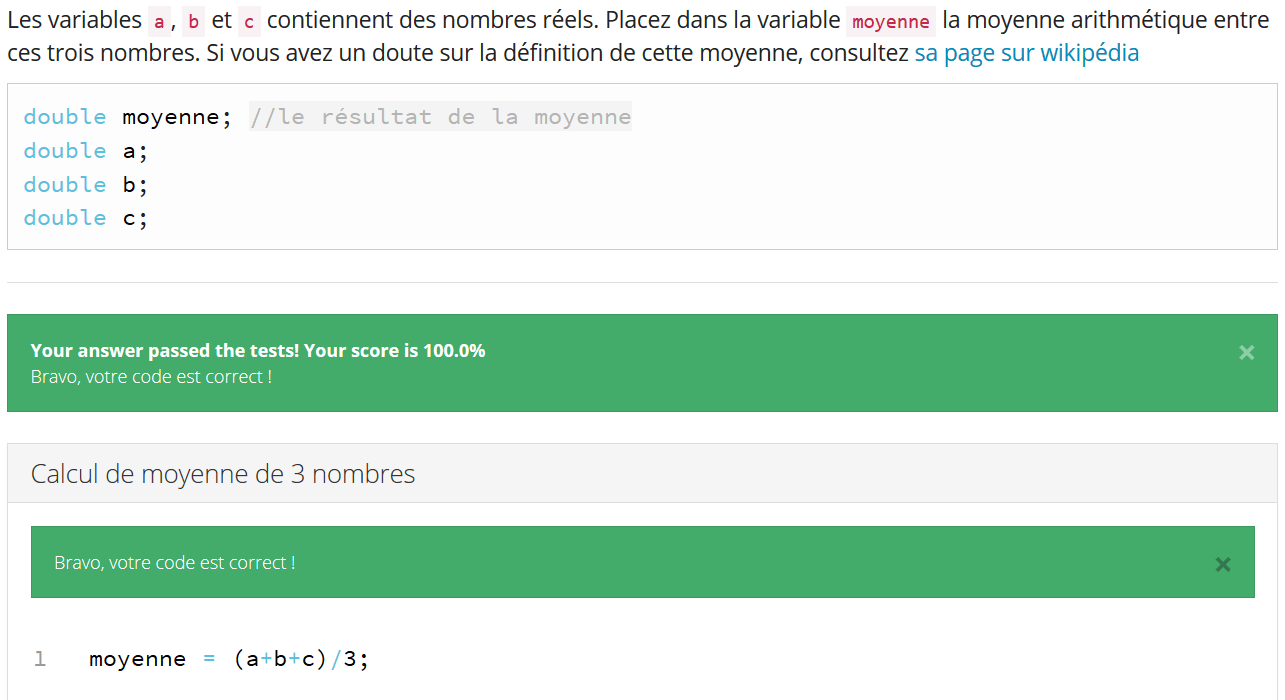
\includegraphics[width=\linewidth]{img/1}
\end{figure}
\pagebreak
\subsubsection{Nombre de secondes depuis minuit}
\begin{figure}[!h]
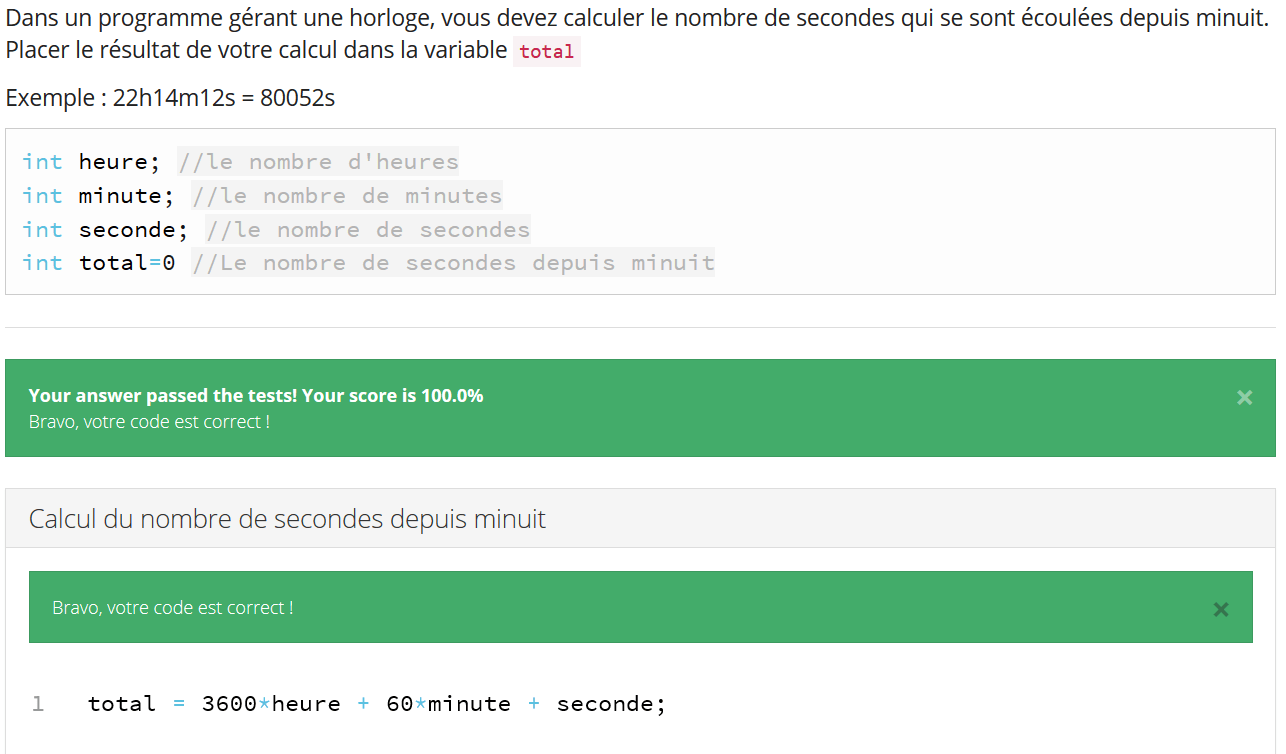
\includegraphics[width=\linewidth]{img/2}
\end{figure}
\pagebreak
\subsubsection{Siècle}
\begin{figure}[!h]
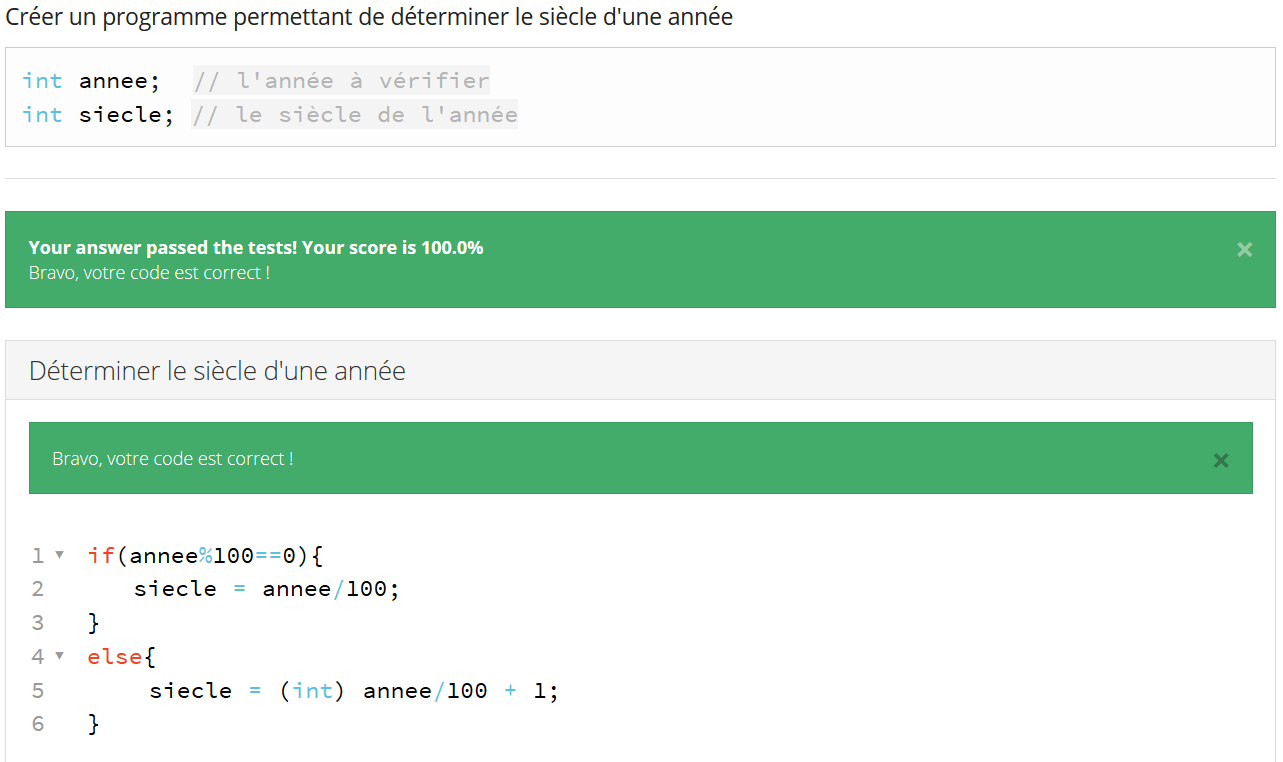
\includegraphics[width=\linewidth]{img/3}
\end{figure}
\newpage
\subsubsection{Indice de Quételet}
\begin{figure}[!h]
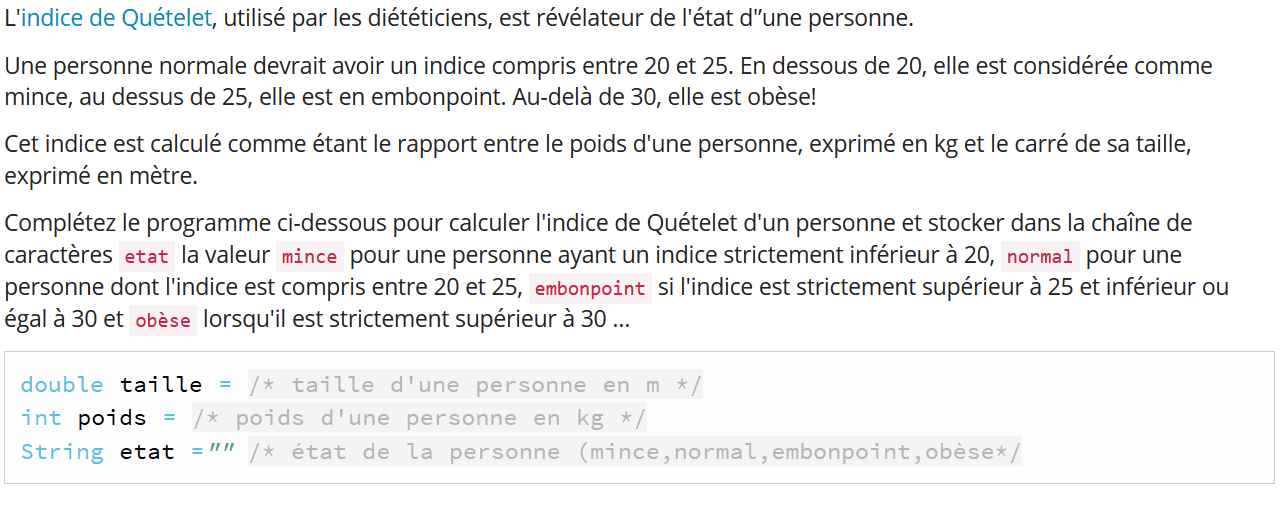
\includegraphics[width=\linewidth]{img/4e}
\end{figure}
\begin{figure}[!h]
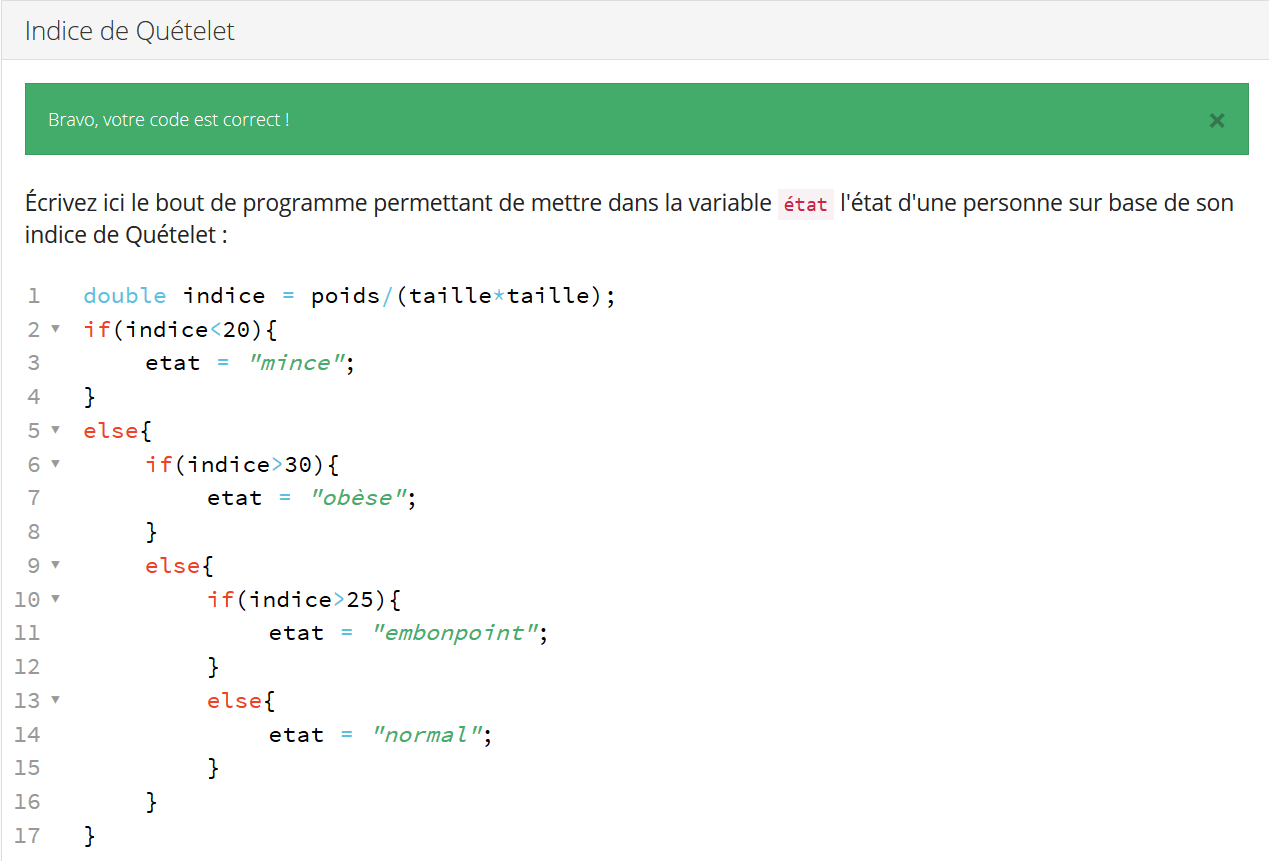
\includegraphics[width=\linewidth]{img/4r}
\end{figure}
\newpage
\subsubsection{Ordonne}
\begin{figure}[!h]
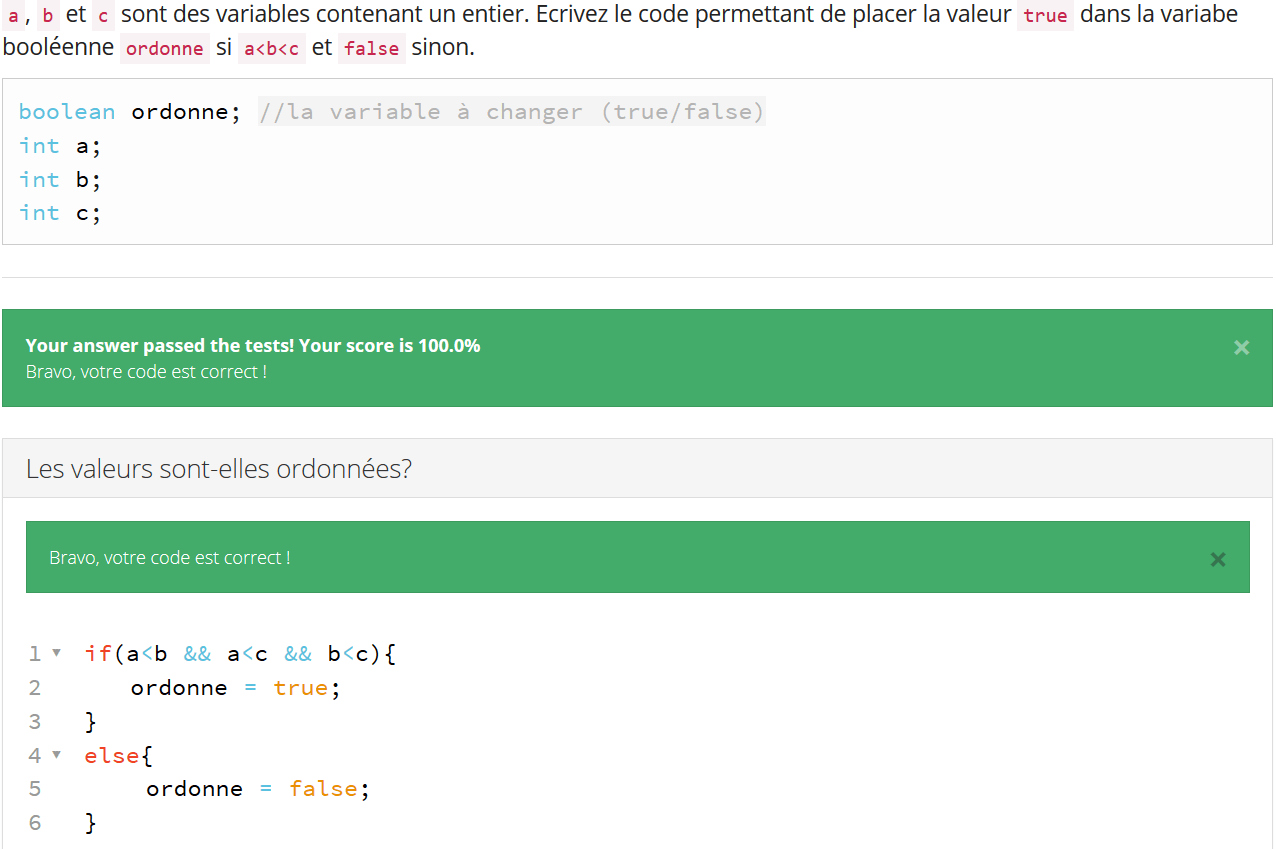
\includegraphics[width=\linewidth]{img/5}
\end{figure}
\newpage
\subsubsection{Année bissextile}
\begin{figure}[!h]
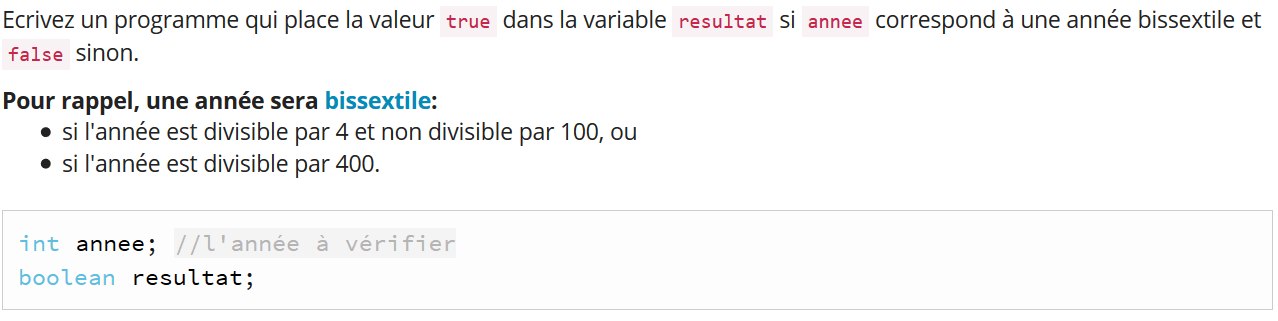
\includegraphics[width=\linewidth]{img/6e}
\end{figure}
\begin{figure}[!h]
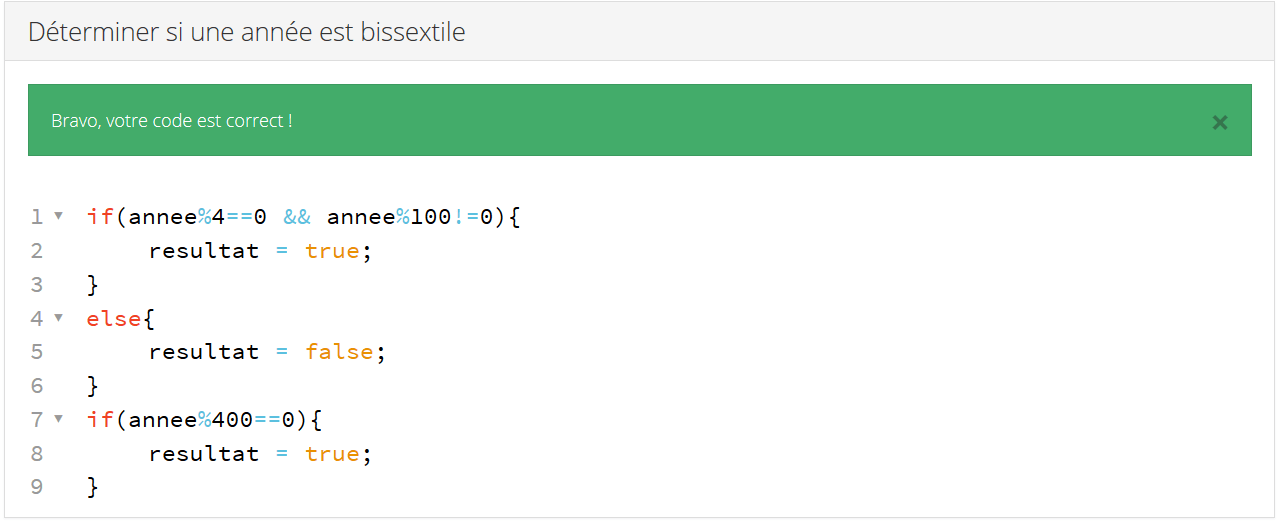
\includegraphics[width=\linewidth]{img/6r}
\end{figure}
\newpage
\subsubsection{Sélecteur de saison}
\begin{figure}[!h]
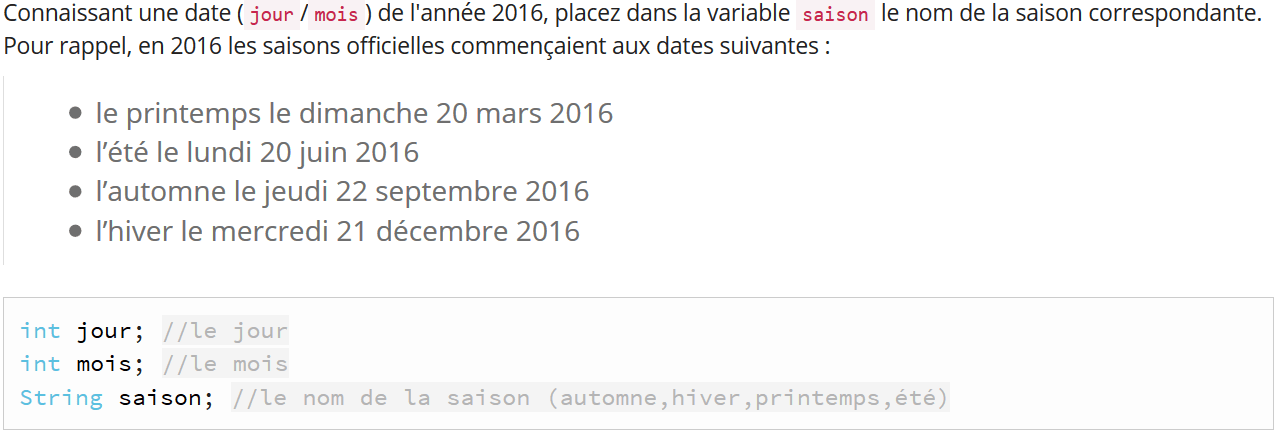
\includegraphics[width=\linewidth]{img/7e}
\end{figure}
\begin{figure}[!h]
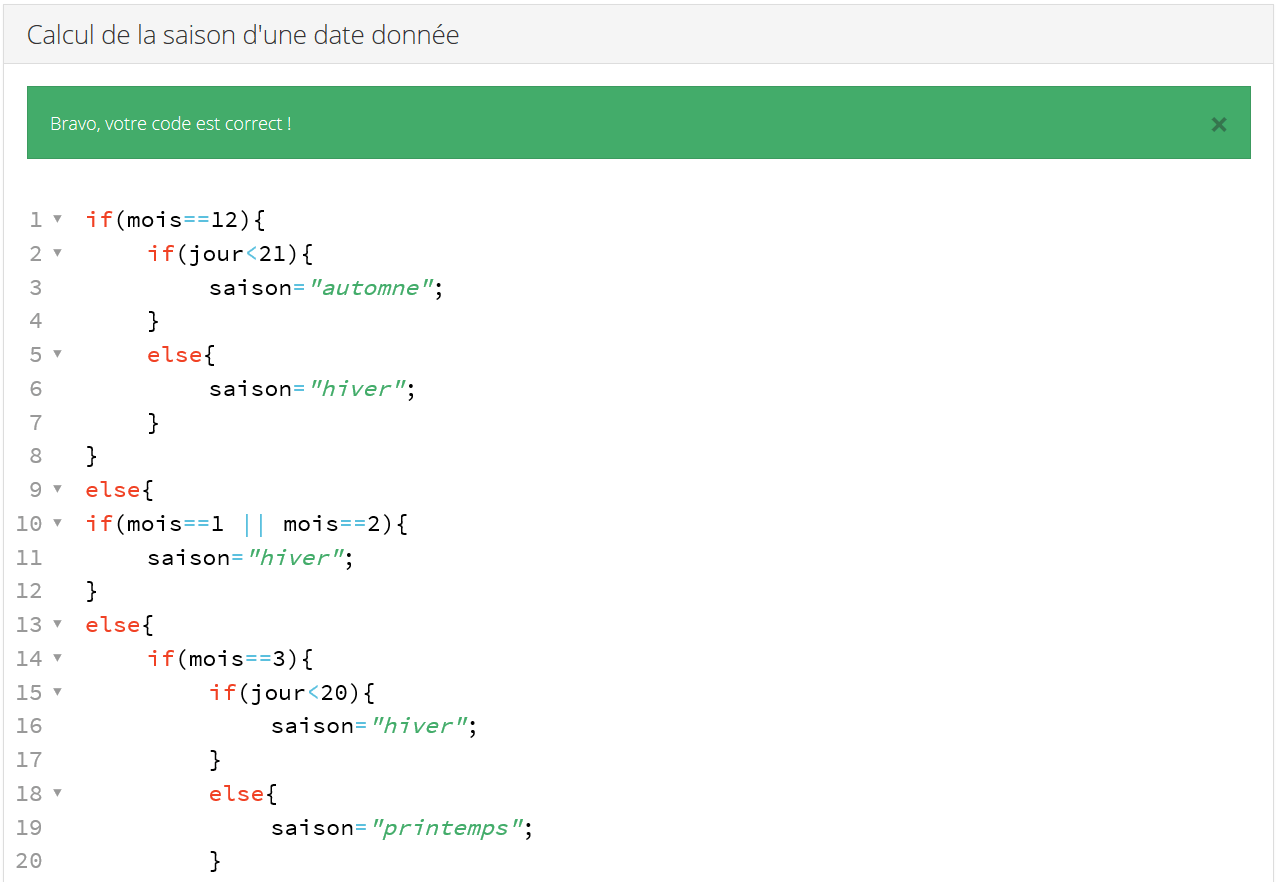
\includegraphics[width=\linewidth]{img/7r1}
\end{figure}
\newpage
\begin{figure}[!h]
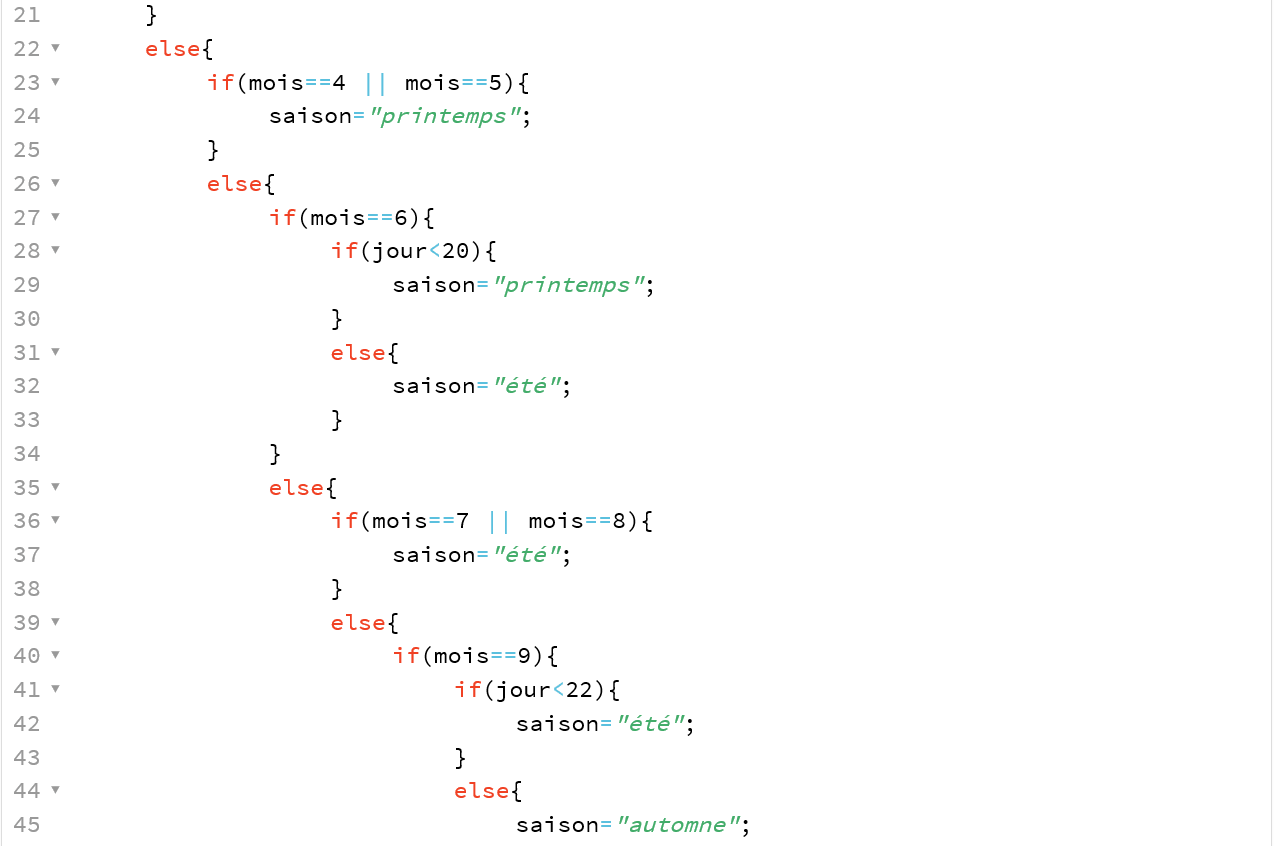
\includegraphics[width=\linewidth]{img/7r2}
\end{figure}
\begin{figure}[!h]
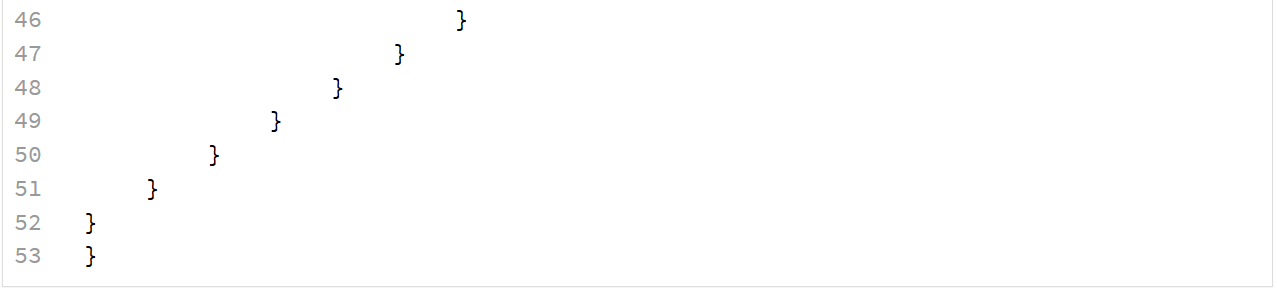
\includegraphics[width=\linewidth]{img/7r3}
\end{figure}
\newpage
\subsubsection{Maximum}
\begin{figure}[!h]
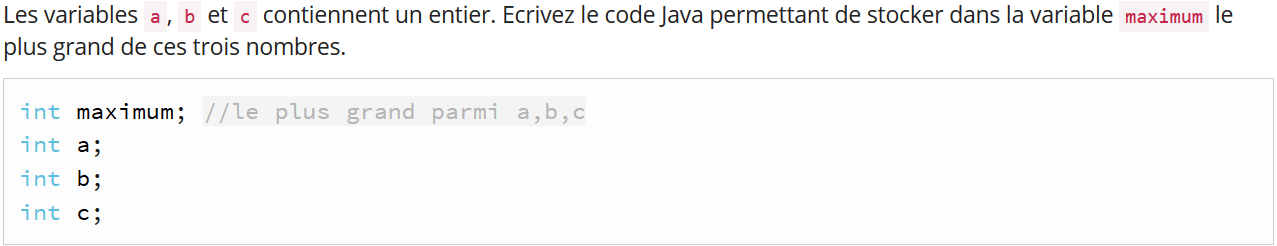
\includegraphics[width=\linewidth]{img/8e}
\end{figure}
\begin{figure}[!h]
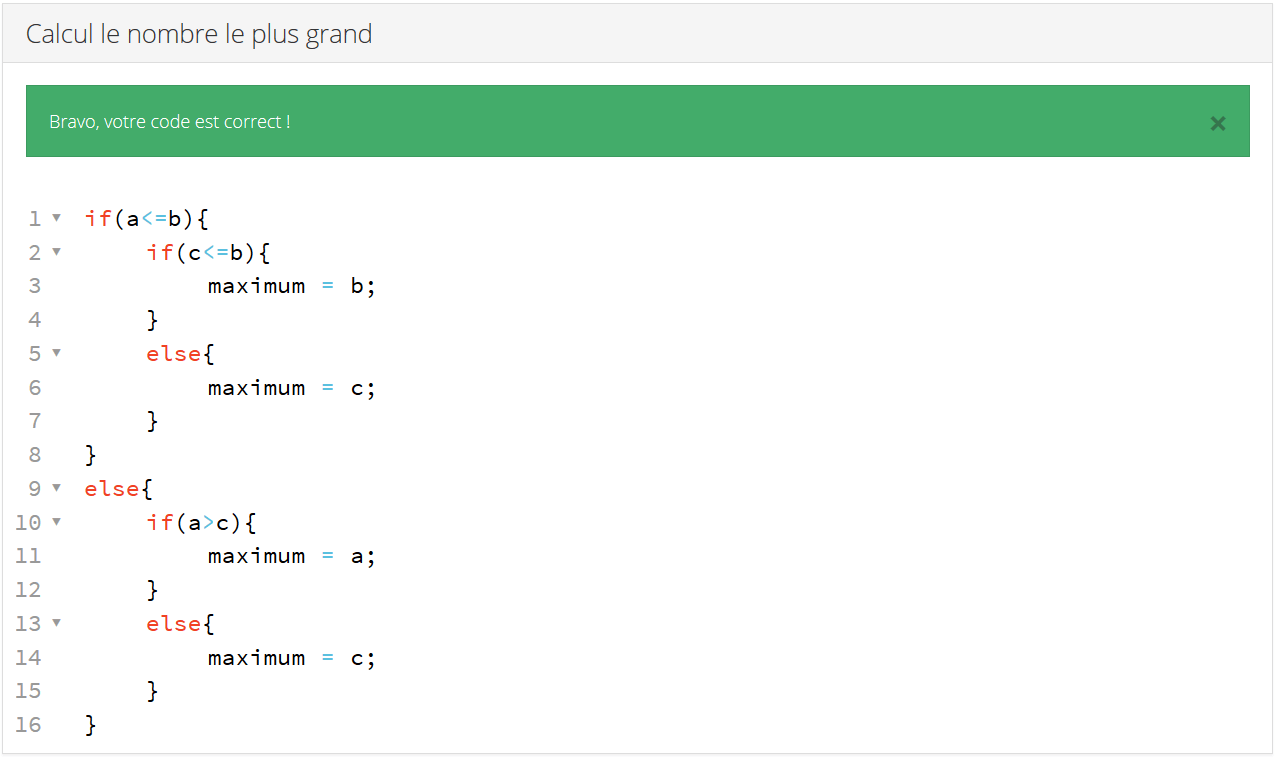
\includegraphics[width=\linewidth]{img/8r}
\end{figure}
\newpage
\subsubsection{Minimum}
\begin{figure}[!h]
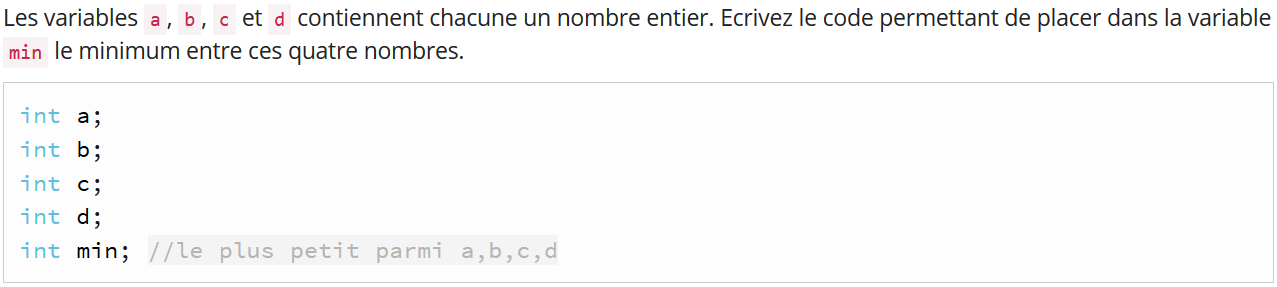
\includegraphics[width=\linewidth]{img/9e}
\end{figure}
\begin{figure}[!h]
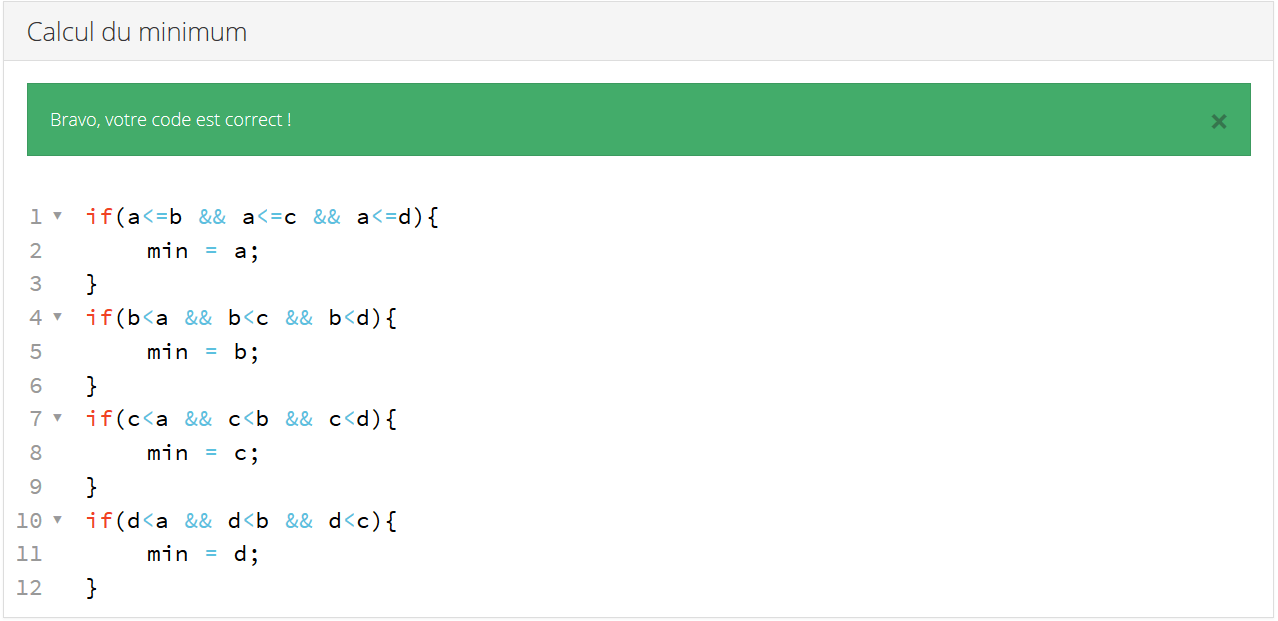
\includegraphics[width=\linewidth]{img/9r}
\end{figure}
\newpage
\subsubsection{Compteur de différence}
\begin{figure}[!h]
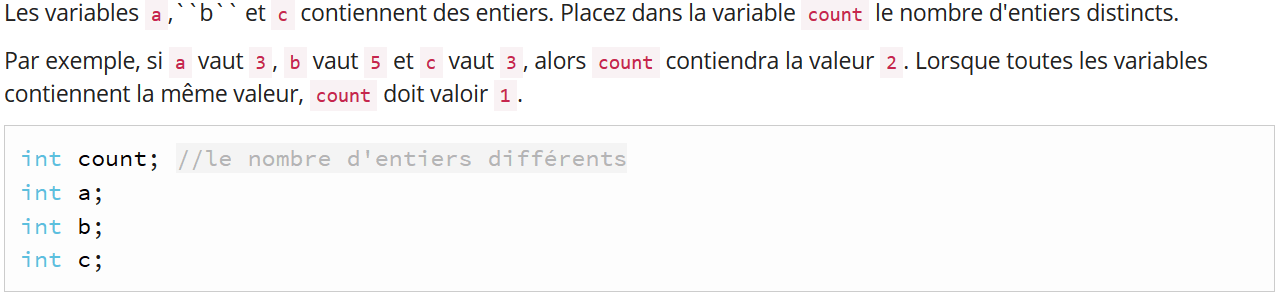
\includegraphics[width=\linewidth]{img/10e}
\end{figure}
\begin{figure}[!h]
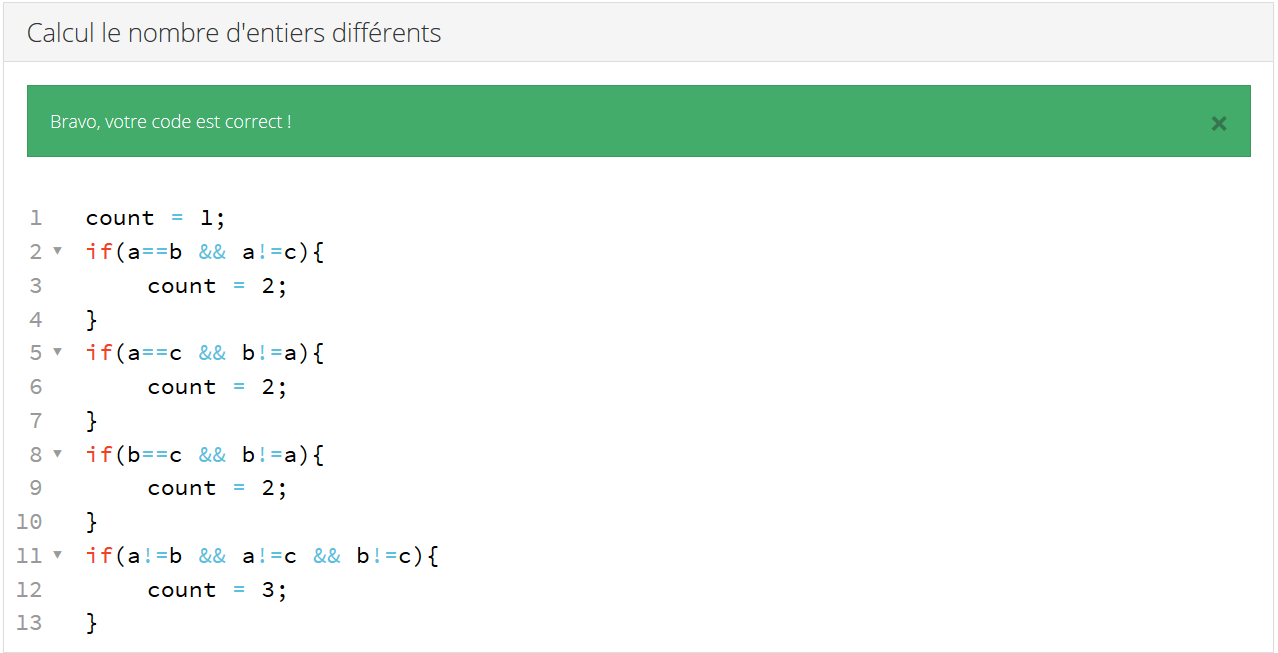
\includegraphics[width=\linewidth]{img/10r}
\end{figure}
\newpage
\subsubsection{Caractère}
\begin{figure}[!h]
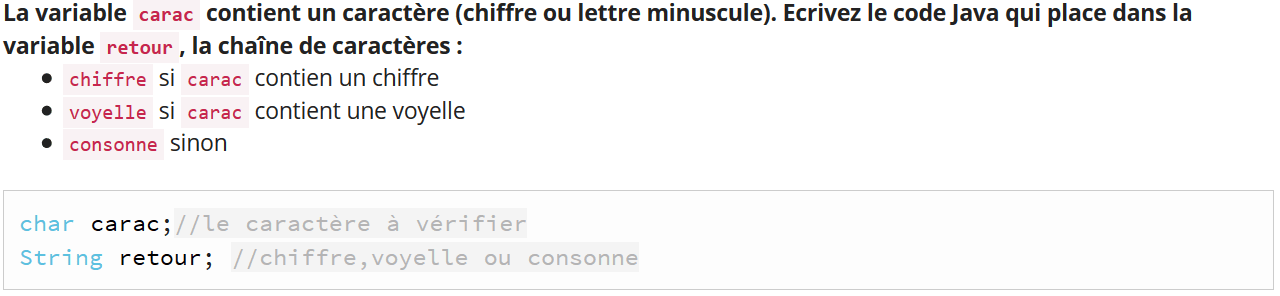
\includegraphics[width=\linewidth]{img/11e}
\end{figure}
\begin{figure}[!h]
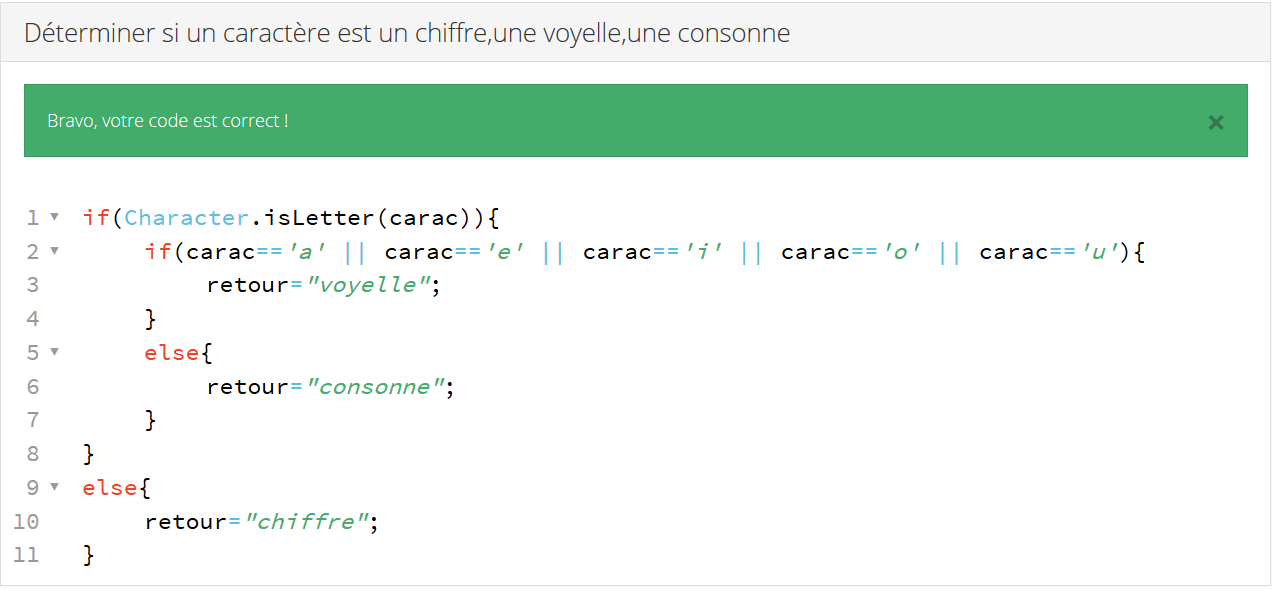
\includegraphics[width=\linewidth]{img/11r}
\end{figure}
\newpage
\subsubsection{Calcul de prix}
\begin{figure}[!h]
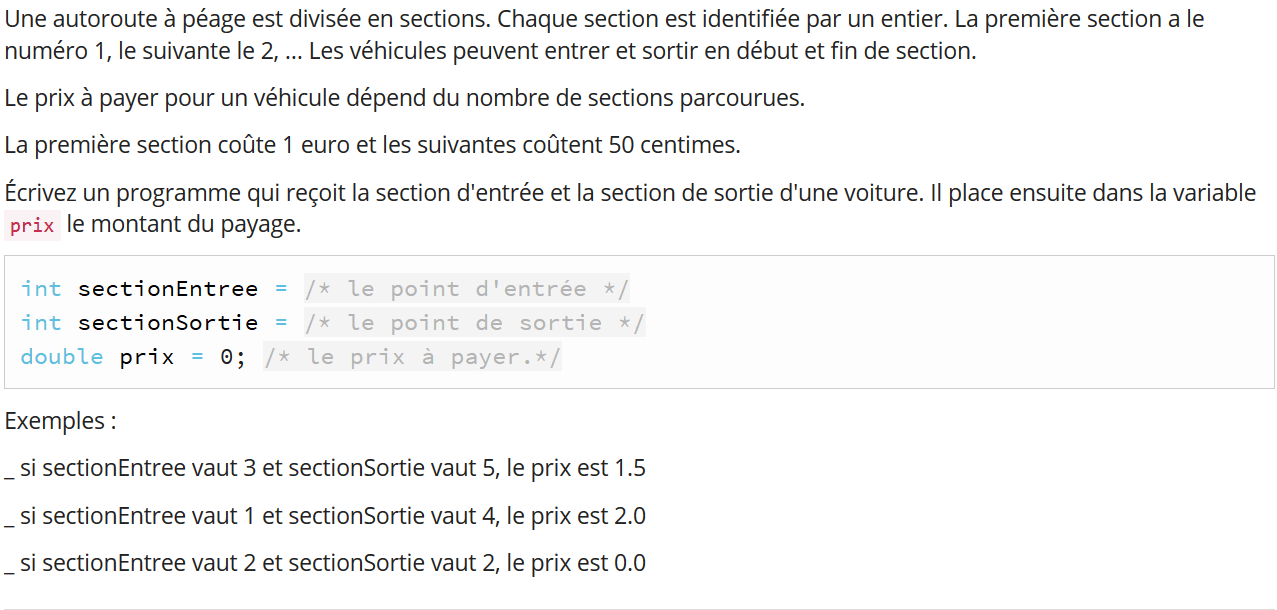
\includegraphics[width=\linewidth]{img/12e}
\end{figure}
\begin{figure}[!h]
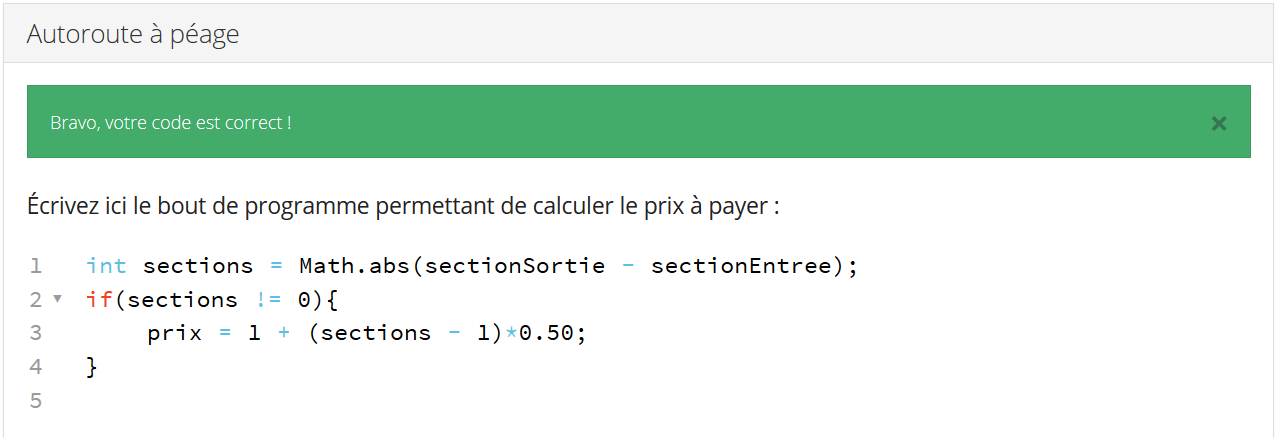
\includegraphics[width=\linewidth]{img/12r}
\end{figure}
\newpage
\subsubsection{Médiane}
\begin{figure}[!h]
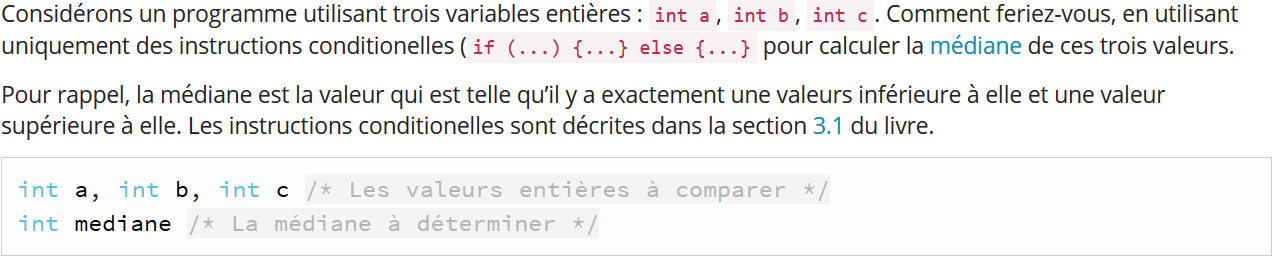
\includegraphics[width=\linewidth]{img/13e}
\end{figure}
\begin{figure}[!h]
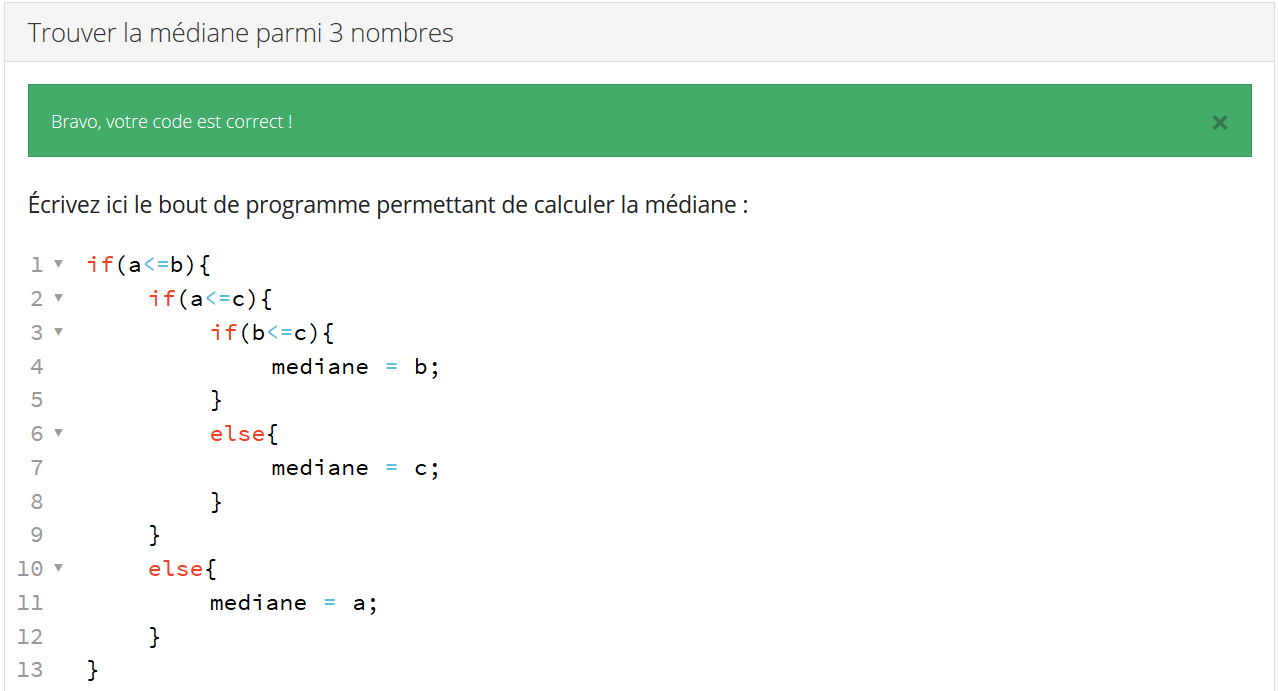
\includegraphics[width=\linewidth]{img/13r1}
\end{figure}
\begin{figure}[!h]
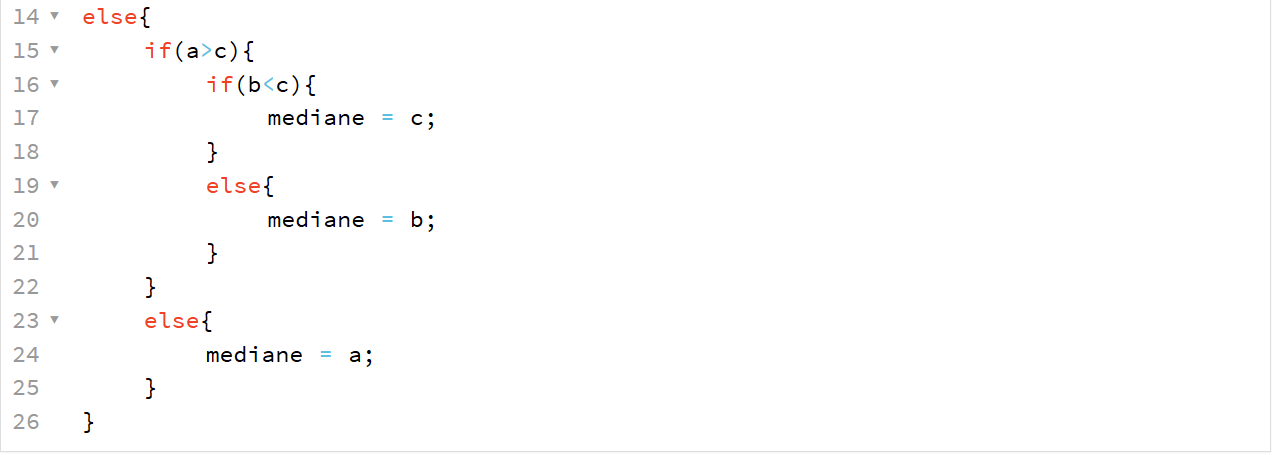
\includegraphics[width=\linewidth]{img/13r2}
\end{figure}
\newpage
\subsubsection{Fizzbuzz}
\begin{figure}[!h]
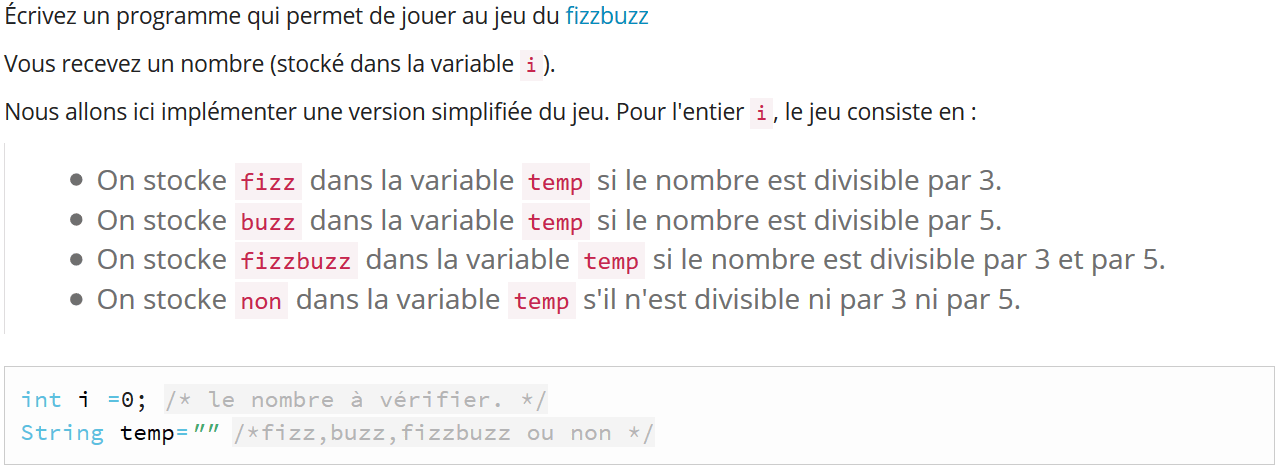
\includegraphics[width=\linewidth]{img/14e}
\end{figure}
\begin{figure}[!h]
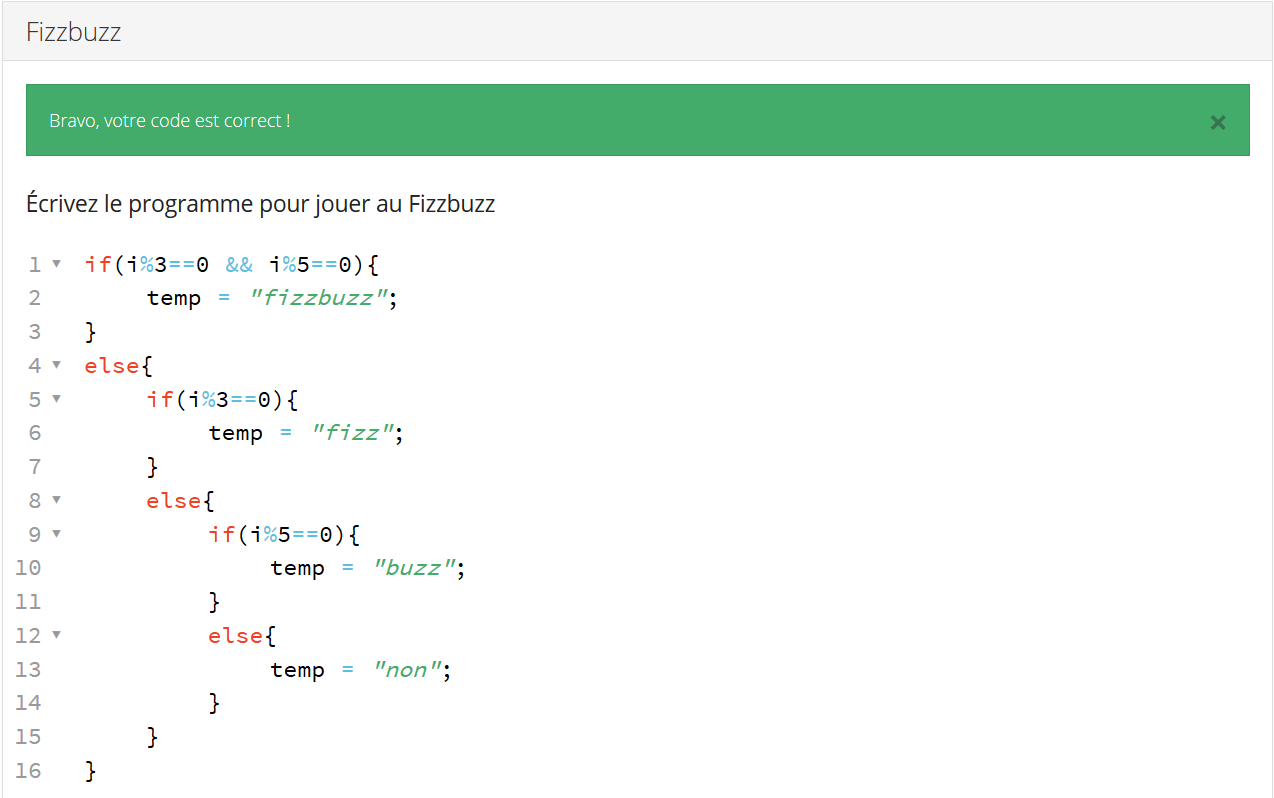
\includegraphics[width=\linewidth]{img/14r}
\end{figure}
\newpage
\subsubsection{OU exclusif}
\begin{figure}[!h]
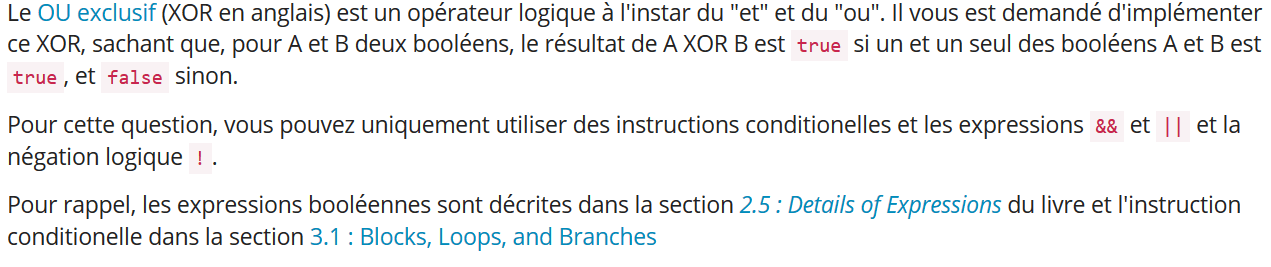
\includegraphics[width=\linewidth]{img/15e}
\end{figure}
\begin{figure}[!h]
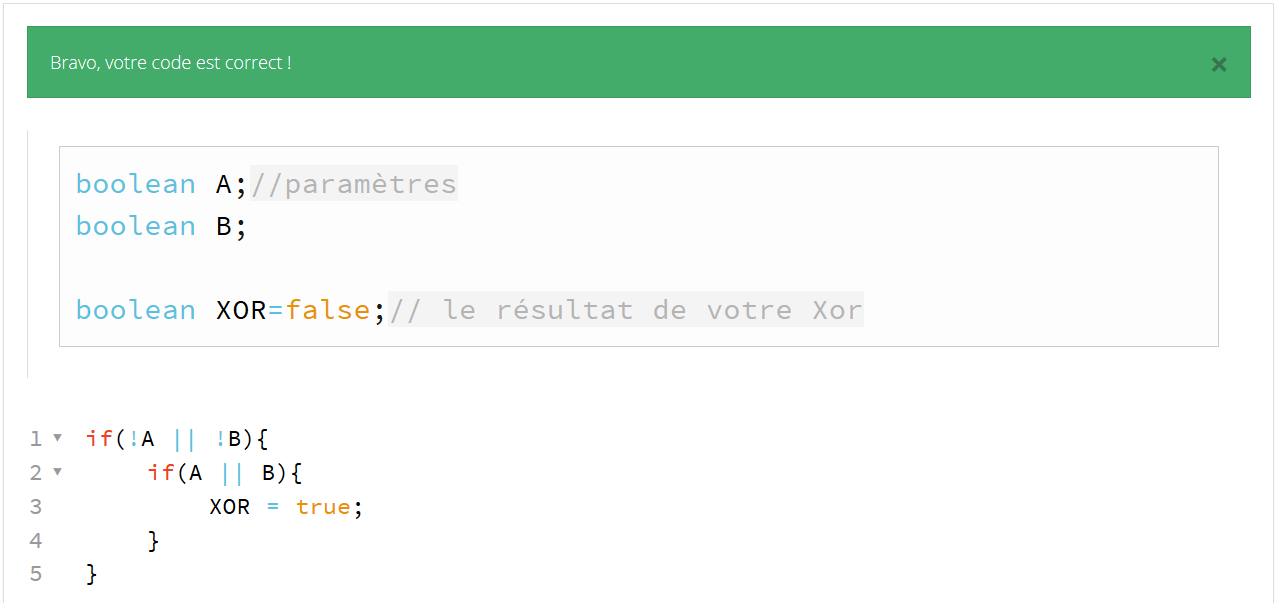
\includegraphics[width=\linewidth]{img/15r}
\end{figure}
\newpage
\subsubsection{Calcul d'amende}
\begin{figure}[!h]
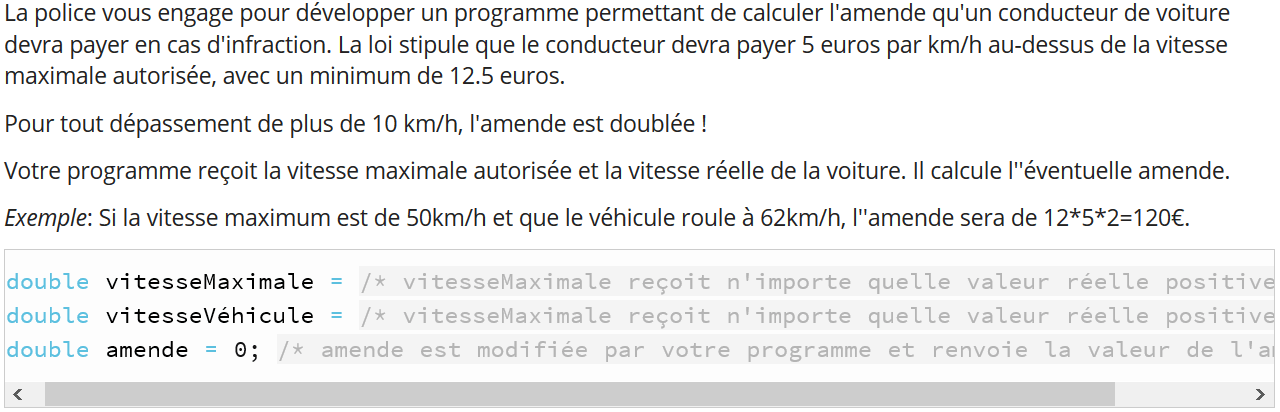
\includegraphics[width=\linewidth]{img/16e}
\end{figure}
\begin{figure}[!h]
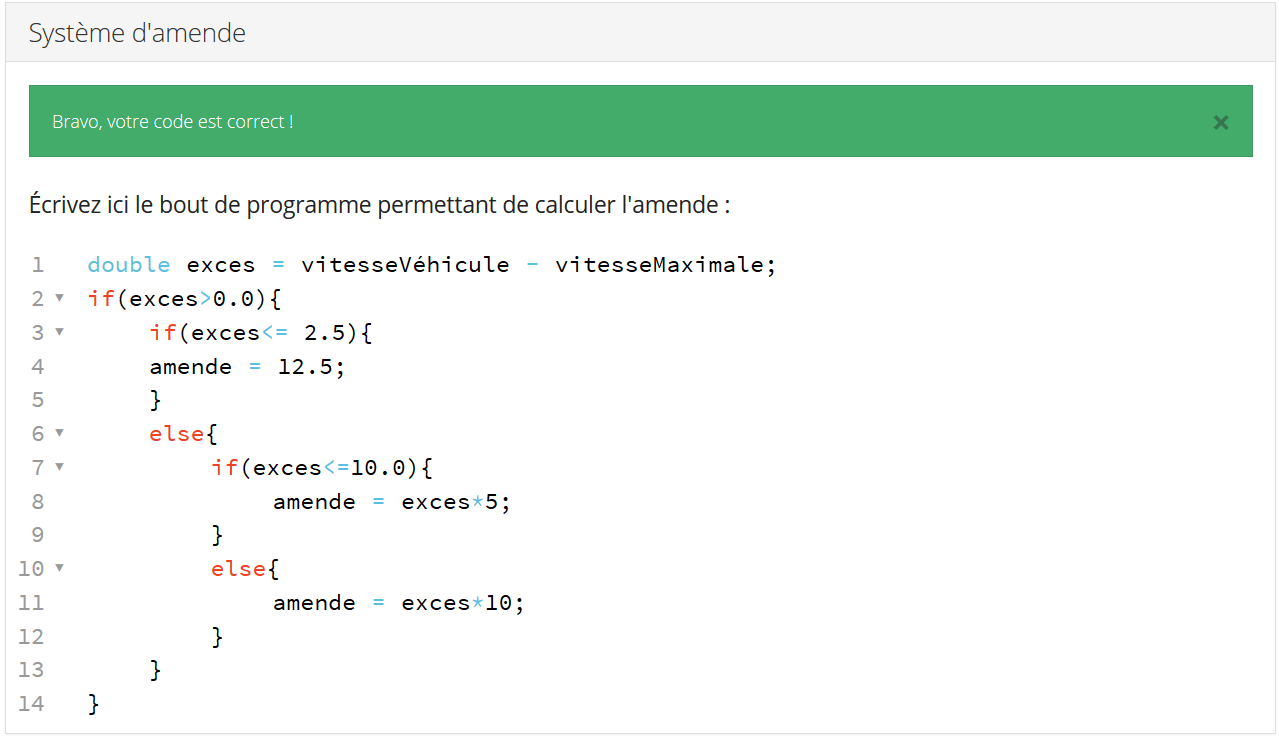
\includegraphics[width=\linewidth]{img/16r}
\end{figure}
\newpage
\subsubsection{Somme d'entiers pairs}
\begin{figure}[!h]
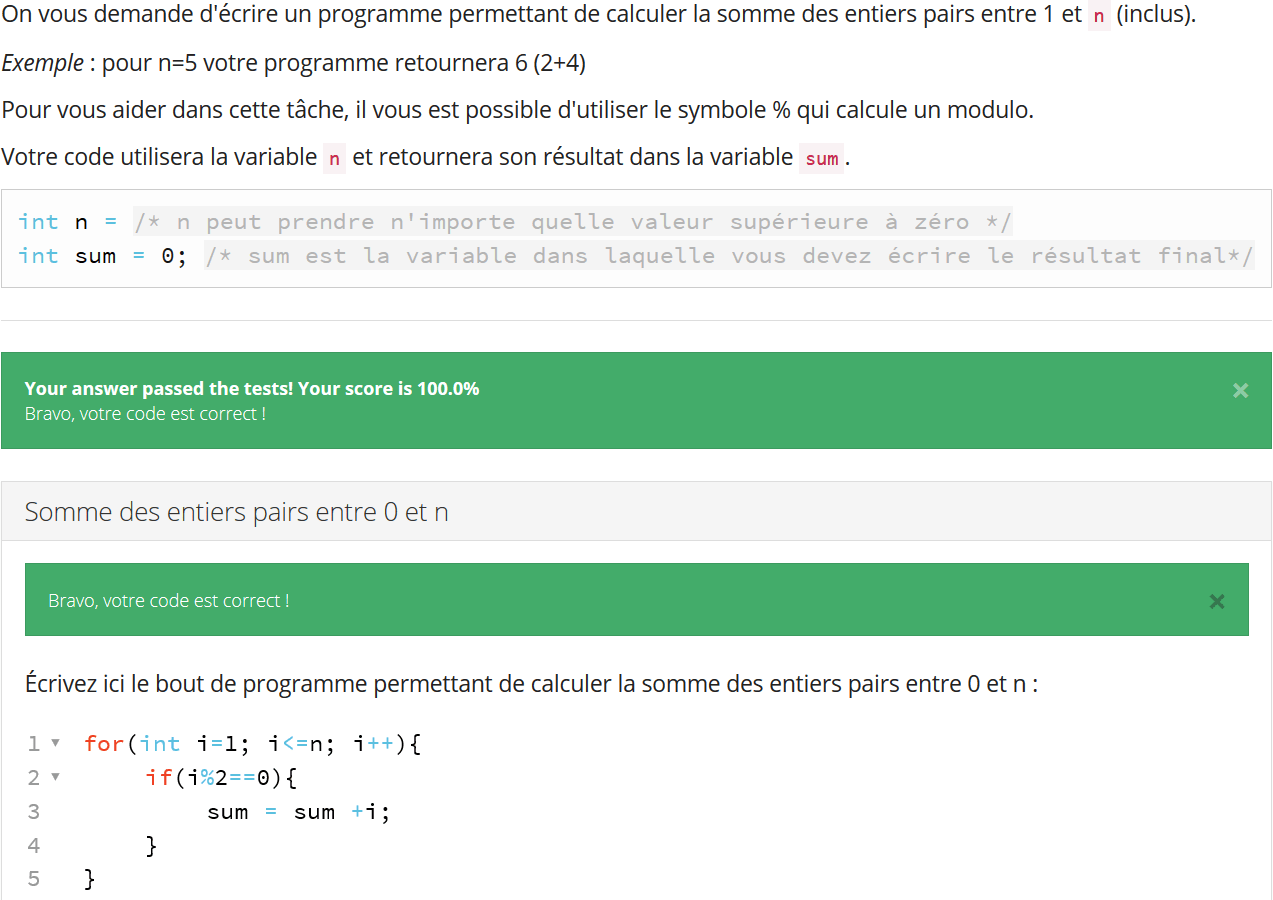
\includegraphics[width=\linewidth]{img/17}
\end{figure}
\newpage
\subsubsection{IN/OUT}
\begin{figure}[!h]
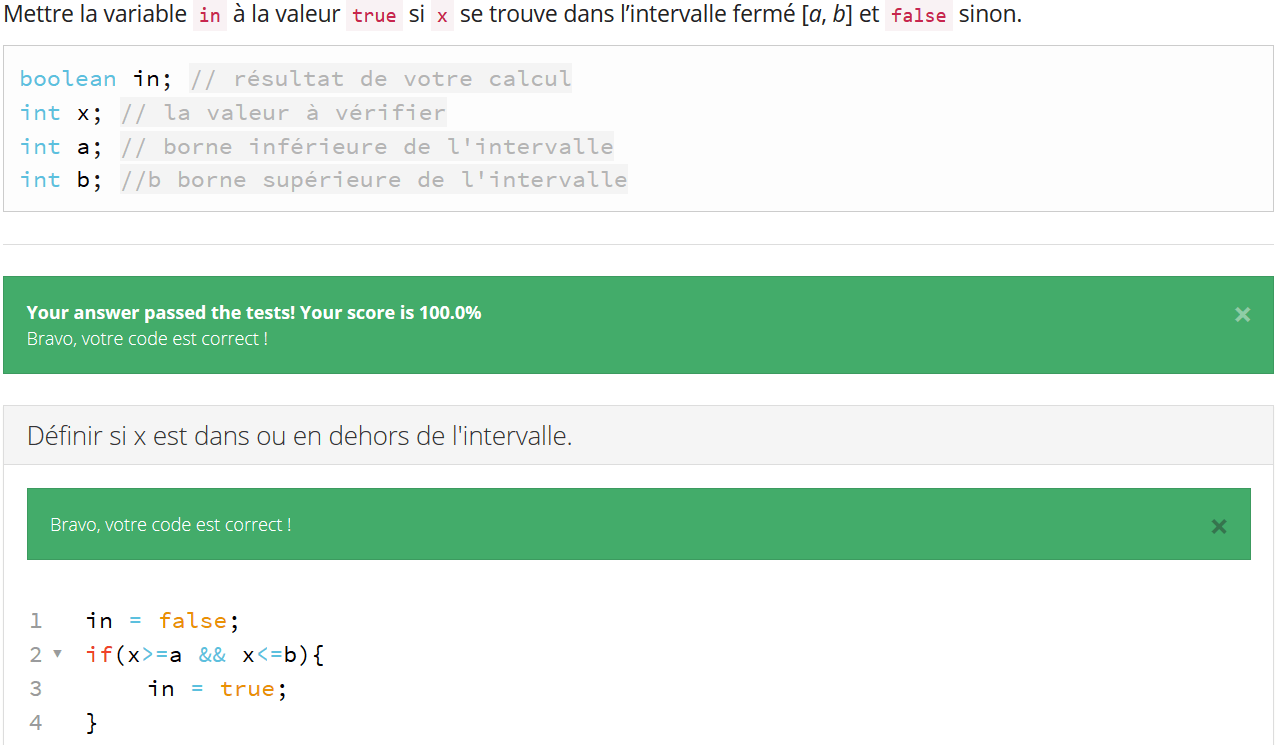
\includegraphics[width=\linewidth]{img/18}
\end{figure}
\newpage
\subsection{Question de bilan final}
\begin{figure}[!h]
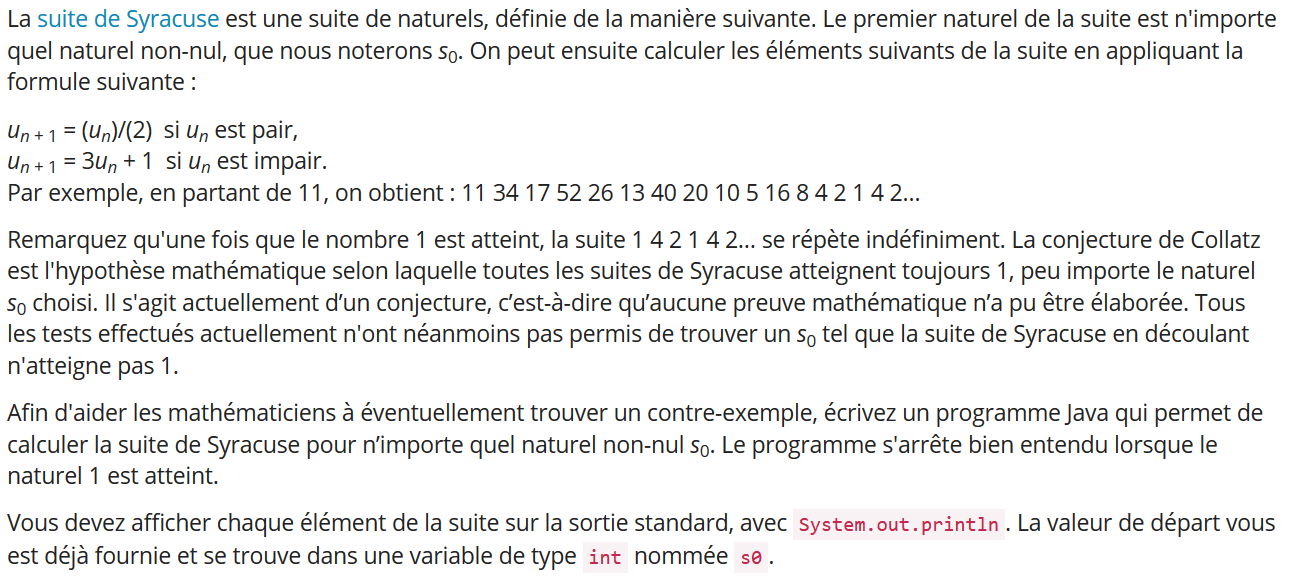
\includegraphics[width=\linewidth]{img/19e}
\end{figure}
\begin{figure}[!h]
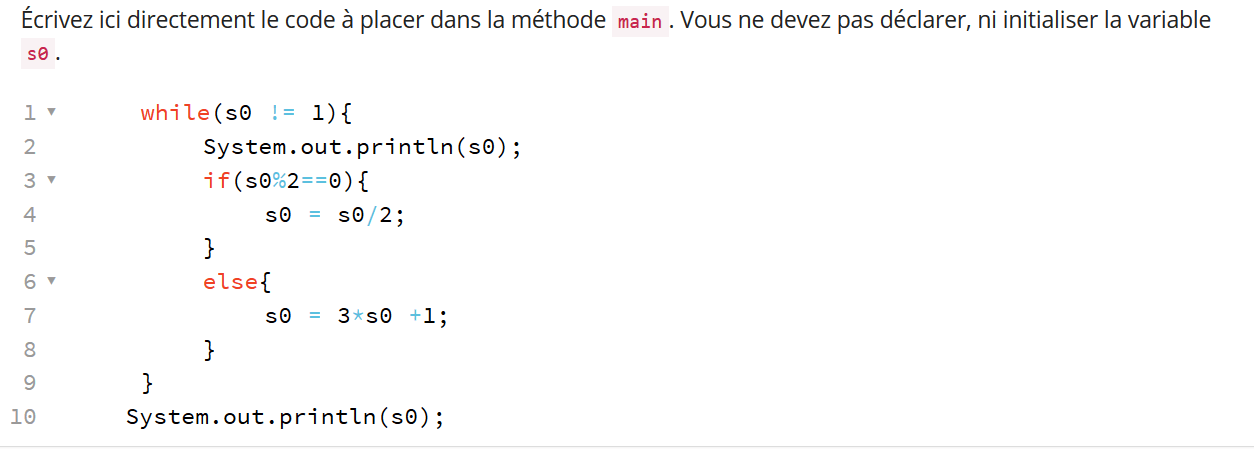
\includegraphics[width=\linewidth]{img/19r}
\end{figure}
\newpage
\section{Mission 2}
\subsection{Questions de démarrage}
\subsubsection{Les bases}
\begin{figure}[!h]
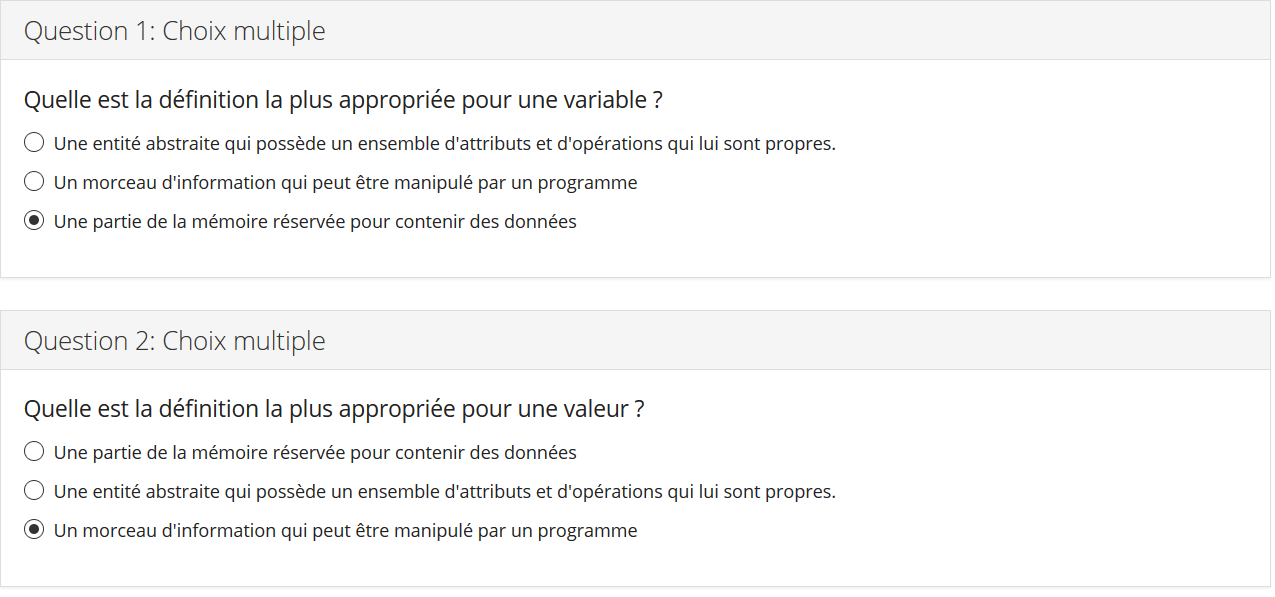
\includegraphics[width=\linewidth]{img/20r1}
\end{figure}
\begin{figure}[!h]
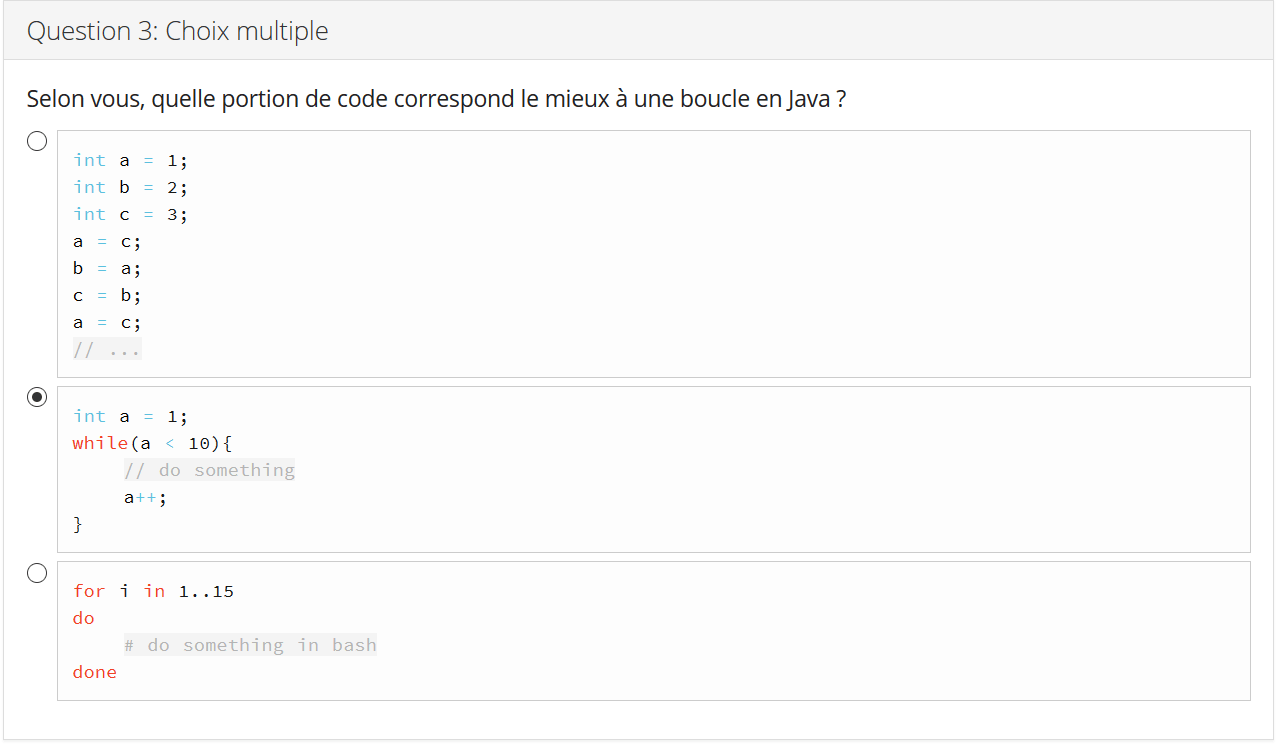
\includegraphics[width=\linewidth]{img/20r2}
\end{figure}
\newpage
\begin{figure}[!h]
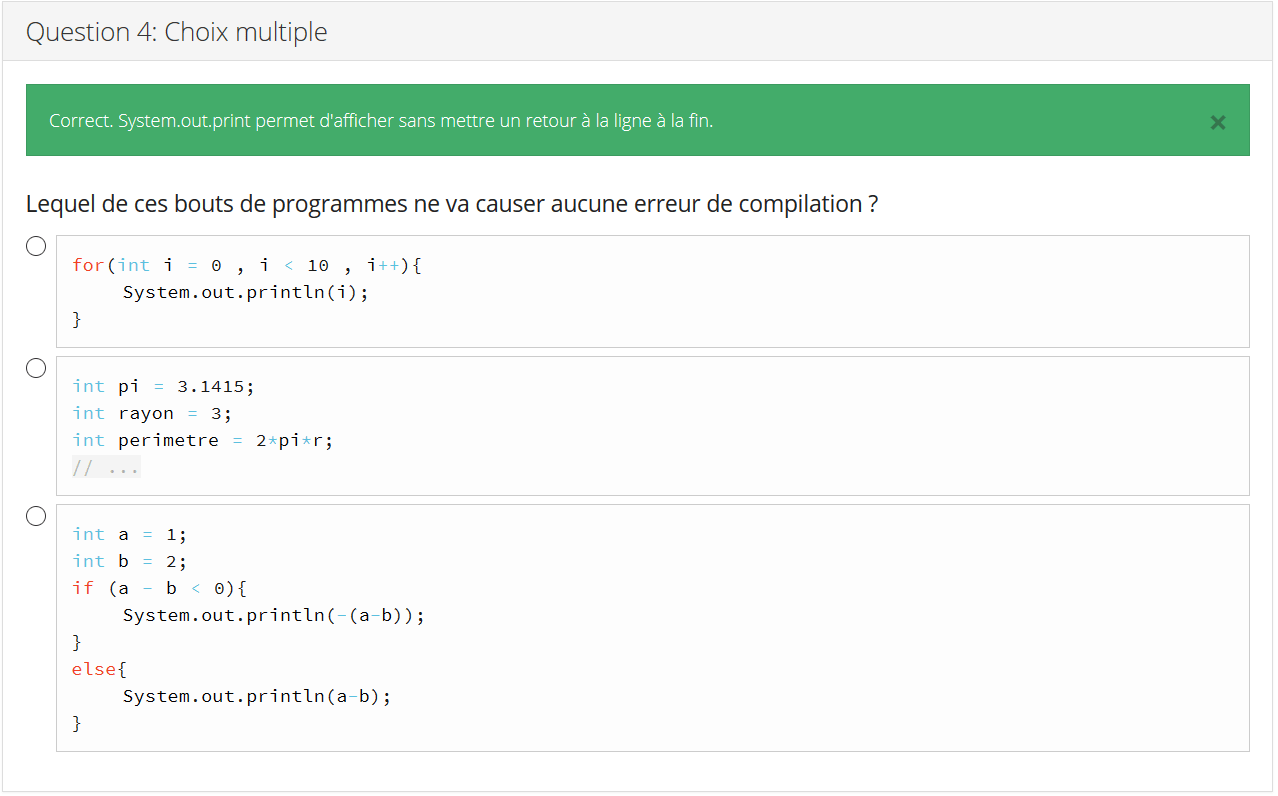
\includegraphics[width=\linewidth]{img/20r3}
\end{figure}
\newpage
\subsubsection{Somme d'entiers}
\begin{figure}[!h]
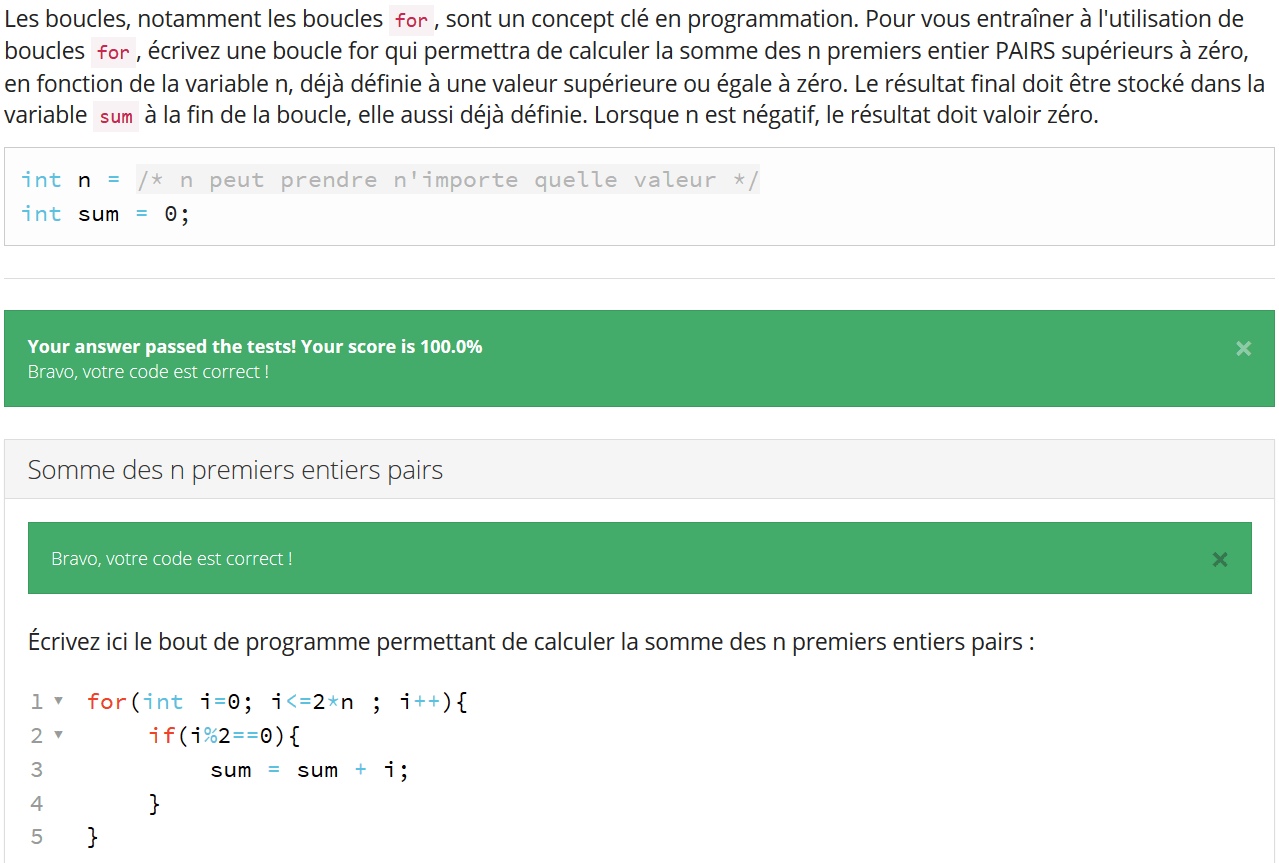
\includegraphics[width=\linewidth]{img/21}
\end{figure}
\newpage
\subsubsection{Puissances}
\begin{figure}[!h]
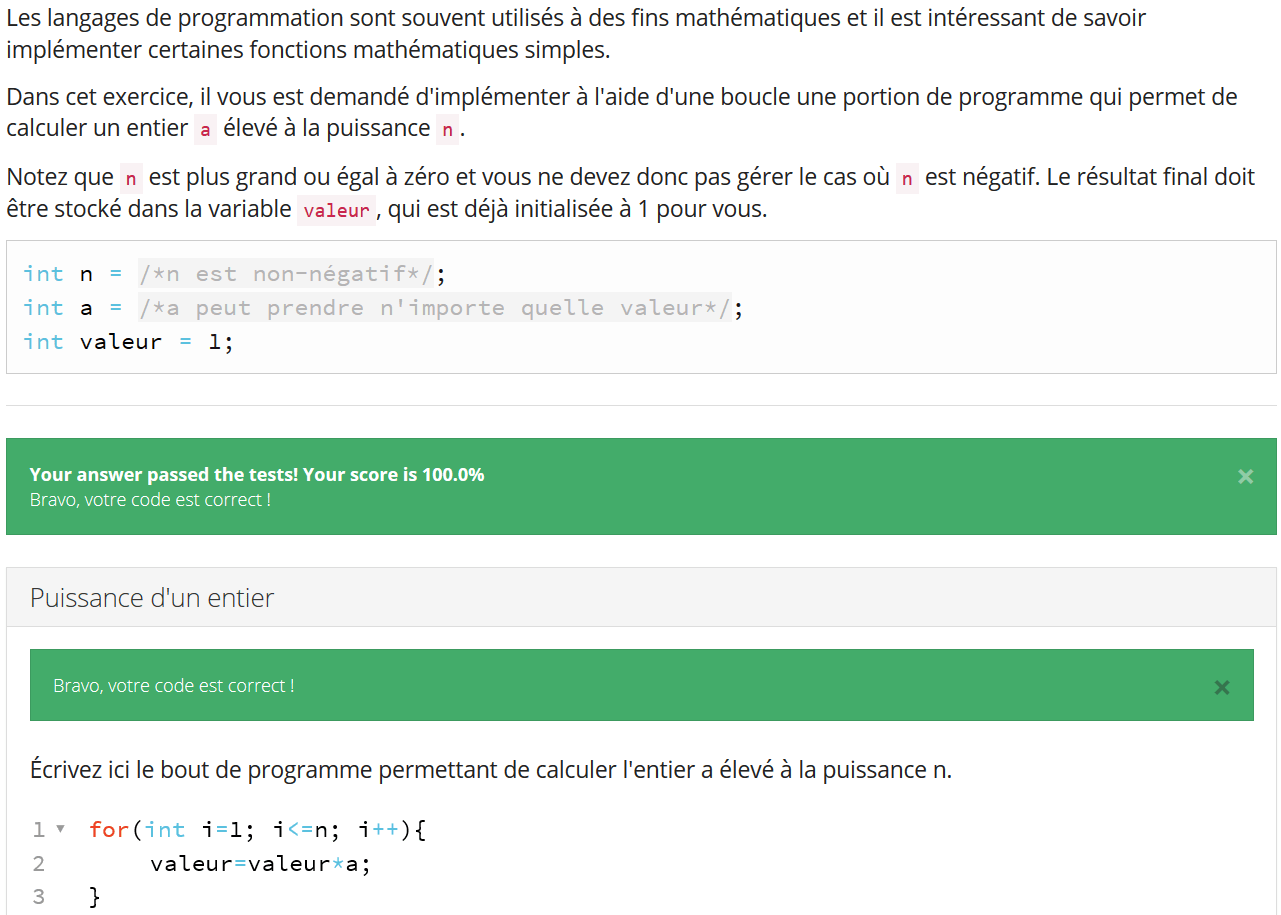
\includegraphics[width=\linewidth]{img/22}
\end{figure}
\newpage
\subsubsection{Plus grand diviseur}
\begin{figure}[!h]
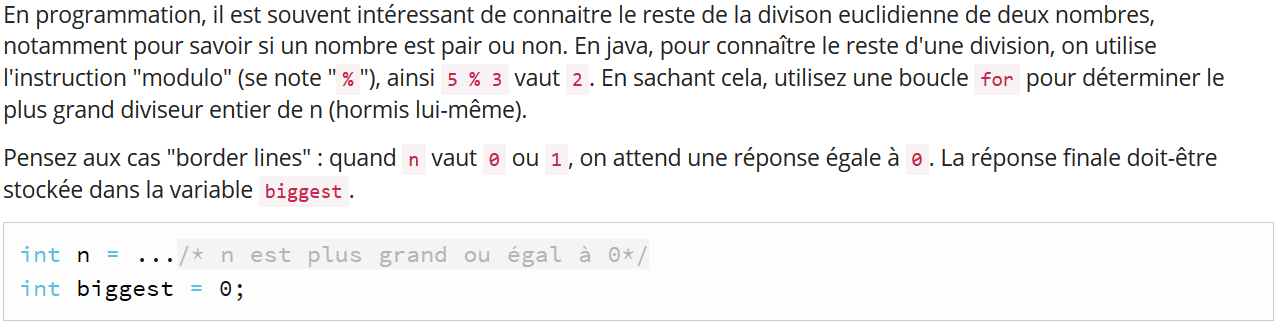
\includegraphics[width=\linewidth]{img/23e}
\end{figure}
\begin{figure}[!h]
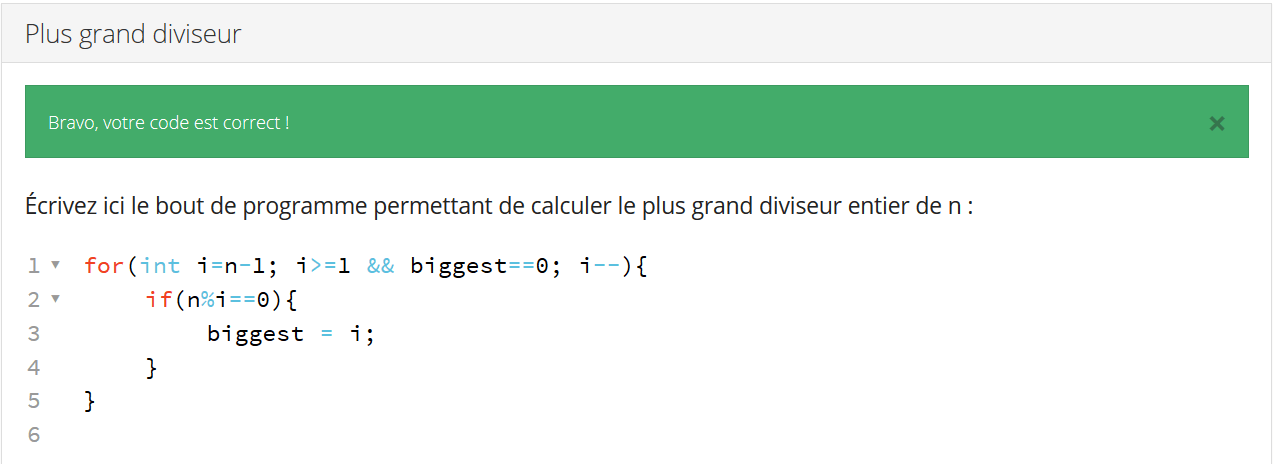
\includegraphics[width=\linewidth]{img/23r}
\end{figure}
\newpage
\subsubsection{Nombres premiers}
\begin{figure}[!h]
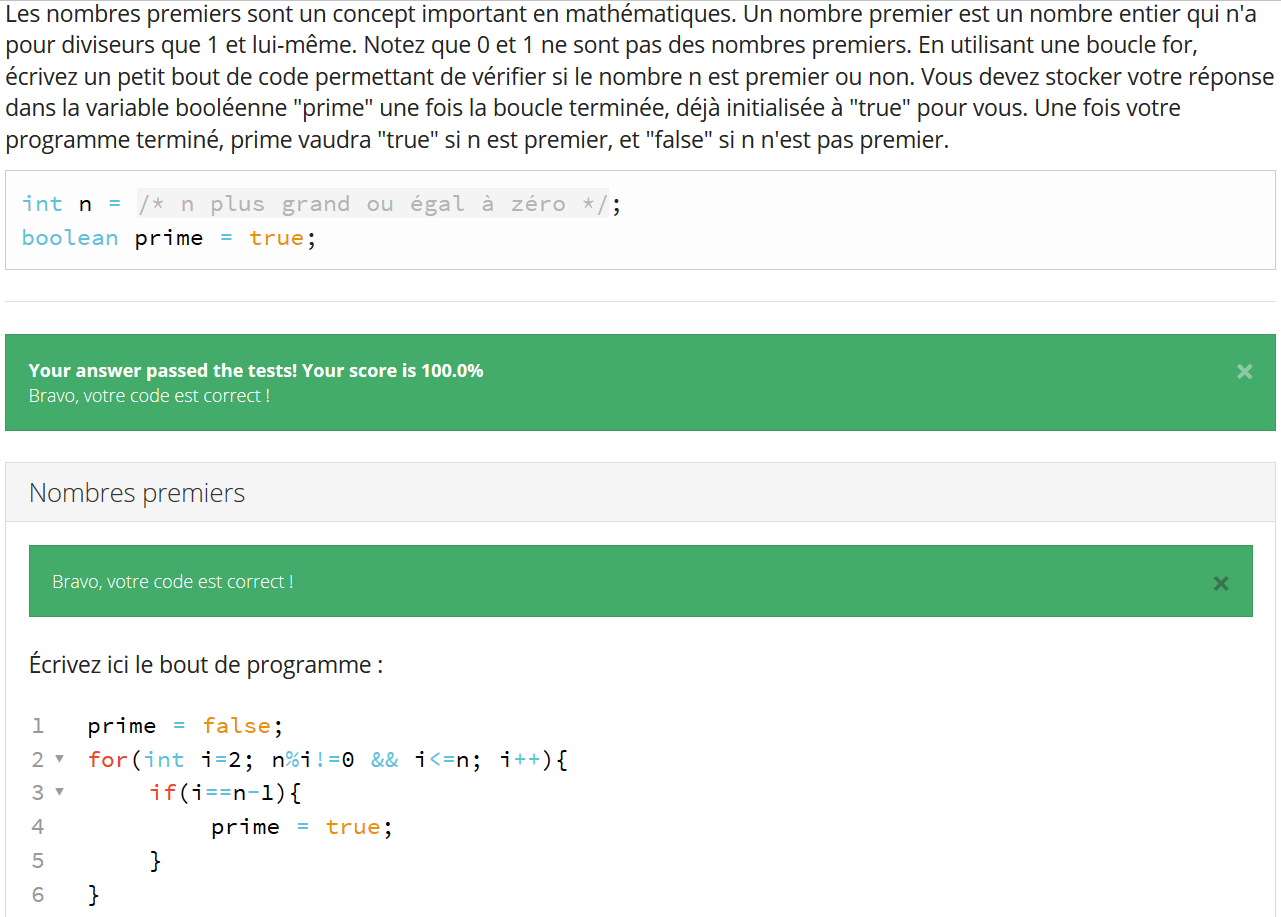
\includegraphics[width=\linewidth]{img/24}
\end{figure}
\newpage
\subsection{Questions supplémentaires}
\subsubsection{Dessin d'un triangle}
\begin{figure}[!h]
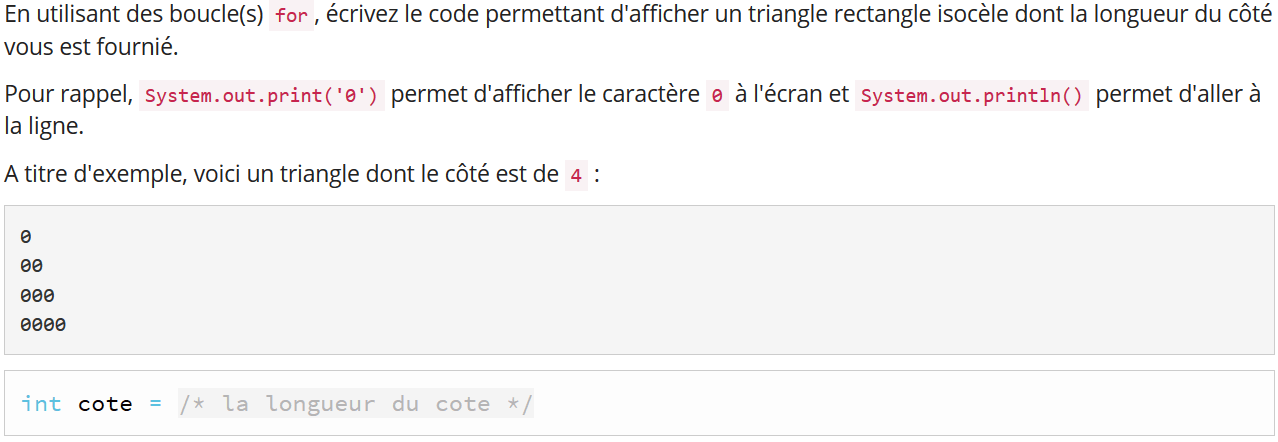
\includegraphics[width=\linewidth]{img/25e}
\end{figure}
\begin{figure}[!h]
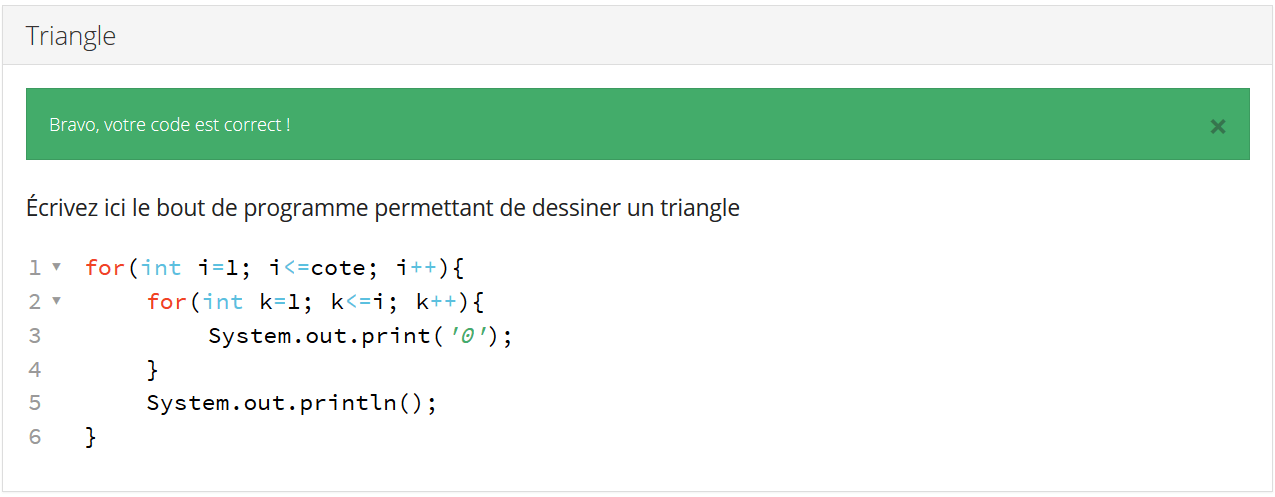
\includegraphics[width=\linewidth]{img/25r}
\end{figure}
\newpage
\subsubsection{Calcul du nombre de diviseurs distincts}
\begin{figure}[!h]
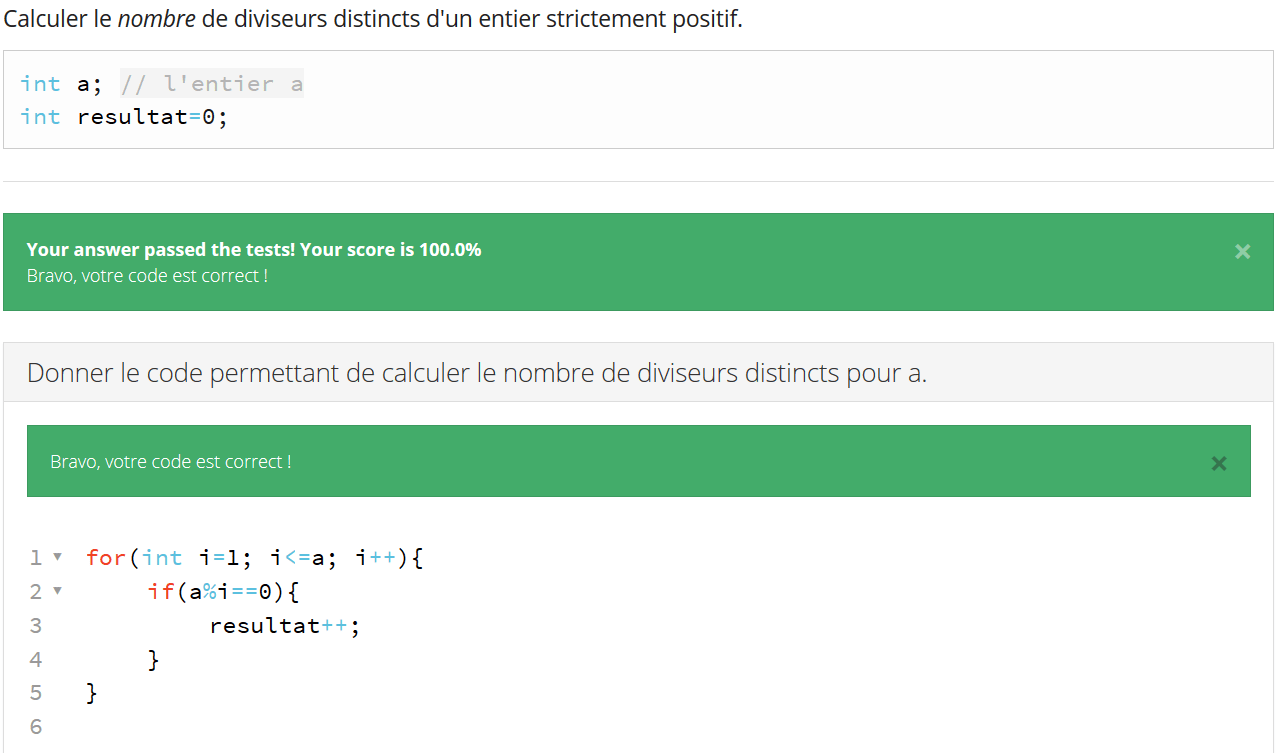
\includegraphics[width=\linewidth]{img/26}
\end{figure}
\newpage
\subsubsection{Dessin de H}
\begin{figure}[!h]
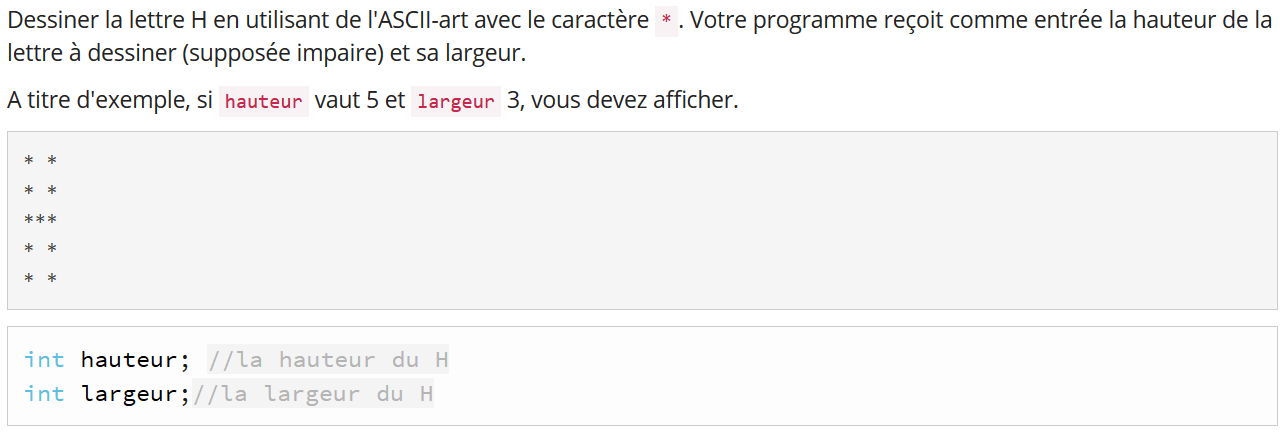
\includegraphics[width=\linewidth]{img/27e}
\end{figure}
\begin{figure}[!h]
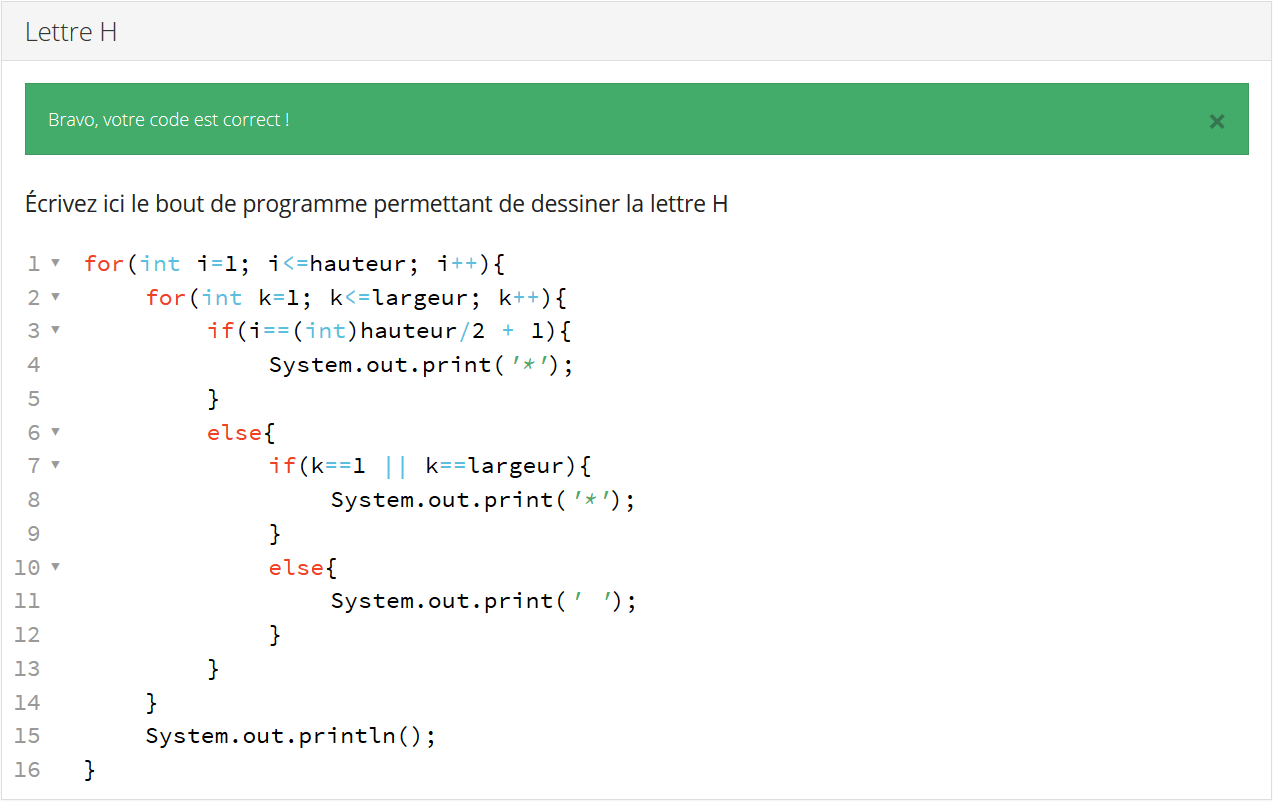
\includegraphics[width=\linewidth]{img/27r}
\end{figure}
\newpage
\subsubsection{Dessin de X}
\begin{figure}[!h]
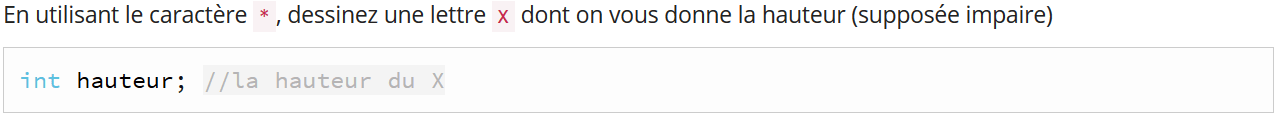
\includegraphics[width=\linewidth]{img/28e}
\end{figure}
\begin{figure}[!h]
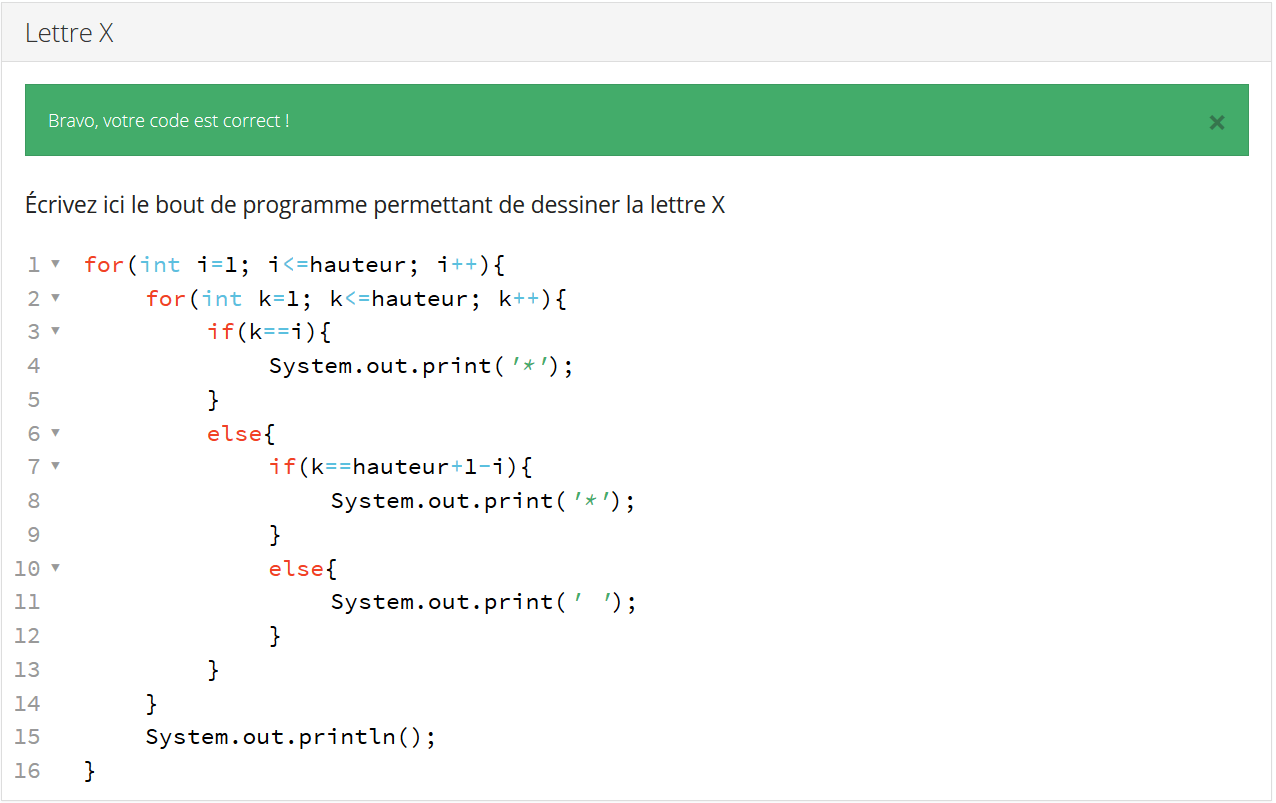
\includegraphics[width=\linewidth]{img/28r}
\end{figure}
\newpage
\subsubsection{Dessin de S}
\begin{figure}[!h]
\includegraphics[width=\linewidth]{img/29r1}
\end{figure}
\begin{figure}[!h]
\includegraphics[width=\linewidth]{img/29r2}
\end{figure}
\newpage
\subsubsection{Calcul de factorielle}
\begin{figure}[!h]
\includegraphics[width=\linewidth]{img/30}
\end{figure}
\newpage
\subsubsection{Somme des entiers entre a et b}
\begin{figure}[!h]
\includegraphics[width=\linewidth]{img/31}
\end{figure}
\newpage
\subsubsection{Calcul d'intérêts}
\begin{figure}[!h]
\includegraphics[width=\linewidth]{img/32}
\end{figure}
\newpage
\subsection{Exercices supplémentaires}
\subsubsection{Calculer le reste d'une division entière}
\begin{figure}[!h]
\includegraphics[width=\linewidth]{img/33}
\end{figure}
\newpage
\subsection{Exercices complémentaires}
\subsubsection{Exercice rapide}
\begin{figure}[!h]
\includegraphics[width=\linewidth]{img/34}
\end{figure}
\newpage
\subsection{Question de bilan final}
\begin{figure}[!h]
\includegraphics[width=\linewidth]{img/35e}
\end{figure}
\begin{figure}[!h]
\includegraphics[width=\linewidth]{img/35r}
\end{figure}
\newpage
\section{Mission 3}
\subsection{Questions de démarrage}
\subsubsection{Conversions}
\begin{figure}[!h]
\includegraphics[width=\linewidth]{img/36e}
\end{figure}
\begin{figure}[!h]
\includegraphics[width=\linewidth]{img/36r}
\end{figure}
\newpage
\subsubsection{Nombre Maximum}
\begin{figure}[!h]
\includegraphics[width=\linewidth]{img/37e}
\end{figure}
\begin{figure}[!h]
\includegraphics[width=\linewidth]{img/37r}
\end{figure}
\newpage
\subsubsection{Nombres Pairs}
\begin{figure}[!h]
\includegraphics[width=\linewidth]{img/38}
\end{figure}
\newpage
\subsubsection{Lettre L}
\begin{figure}[!h]
\includegraphics[width=\linewidth]{img/39e}
\end{figure}
\begin{figure}[!h]
\includegraphics[width=\linewidth]{img/39r}
\end{figure}
\newpage
\subsubsection{Diviseurs Entiers}
\begin{figure}[!h]
\includegraphics[width=\linewidth]{img/40}
\end{figure}
\newpage
\subsection{Exercices Supplémentaires}
\subsubsection{Maximum}
\begin{figure}[!h]
\includegraphics[width=\linewidth]{img/41e}
\end{figure}
\begin{figure}[!h]
\includegraphics[width=\linewidth]{img/41r}
\end{figure}
\newpage
\subsubsection{Calculer la surface d'un rectangle}
\begin{figure}[!h]
\includegraphics[width=\linewidth]{img/42}
\end{figure}
\newpage
\subsubsection{Calculer le volume d'une sphère}
\begin{figure}[!h]
\includegraphics[width=\linewidth]{img/43}
\end{figure}
\newpage
\subsubsection{Intervalle fermé}
\begin{figure}[!h]
\includegraphics[width=\linewidth]{img/44}
\end{figure}
\newpage
\subsubsection{Calcul de la factorielle}
\begin{figure}[!h]
\includegraphics[width=\linewidth]{img/45}
\end{figure}
\newpage
\subsubsection{Carré parfait}
\begin{figure}[!h]
\includegraphics[width=\linewidth]{img/46}
\end{figure}
\newpage
\subsubsection{Médiane}
\begin{figure}[!h]
\includegraphics[width=\linewidth]{img/47e}
\end{figure}
\begin{figure}[!h]
\includegraphics[width=\linewidth]{img/47r}
\end{figure}
\newpage
\subsection{Question de bilan final}
\begin{figure}[!h]
\includegraphics[width=\linewidth-1cm]{img/48e}
\end{figure}
\begin{figure}[!h]
\includegraphics[width=\linewidth-1cm]{img/48r}
\end{figure}
\newpage
\section{Mission 4}
\subsection{Questions de démarrage}
\subsubsection{La classe Character}
\begin{figure}[!h]
\includegraphics[width=\linewidth]{img/49e}
\end{figure}
\begin{figure}[!h]
\includegraphics[width=\linewidth]{img/49r}
\end{figure}
\newpage
\subsubsection{Concaténation}
\begin{figure}[!h]
\includegraphics[width=\linewidth]{img/50e}
\end{figure}
\begin{figure}[!h]
\includegraphics[width=\linewidth]{img/50r}
\end{figure}
\newpage
\subsubsection{Longueur d'un String}
\begin{figure}[!h]
\includegraphics[width=\linewidth]{img/51}
\end{figure}
\newpage
\subsubsection{toUpper}
\begin{figure}[!h]
\includegraphics[width=\linewidth]{img/52e}
\end{figure}
\begin{figure}[!h]
\includegraphics[width=\linewidth]{img/52r}
\end{figure}
\newpage
\subsubsection{Méthode containsChar}
\begin{figure}[!h]
\includegraphics[width=\linewidth]{img/53e}
\end{figure}
\begin{figure}[!h]
\includegraphics[width=\linewidth]{img/53r}
\end{figure}
\newpage
\subsection{Questions supplémentaires}
\subsubsection{Occurences de c dans s}
\begin{figure}[!h]
\includegraphics[width=\linewidth]{img/56}
\end{figure}
\newpage
\subsubsection{Binaire}
\begin{figure}[!h]
\includegraphics[width=\linewidth]{img/57}
\end{figure}
\newpage
\subsubsection{Palindrome}
\begin{figure}[!h]
\includegraphics[width=\linewidth]{img/58}
\end{figure}
\newpage
\subsection{Exercices supplémentaires}
\subsubsection{Caractère dans un String}
\begin{figure}[!h]
\includegraphics[width=\linewidth]{img/54}
\end{figure}
\newpage
\subsubsection{Chaîne composée de chiffres}
\begin{figure}[!h]
\includegraphics[width=\linewidth]{img/55e}
\end{figure}
\begin{figure}[!h]
\includegraphics[width=\linewidth]{img/55r}
\end{figure}
\newpage
\subsubsection{Caractère le plus fréquent}
\begin{figure}[!h]
\includegraphics[width=\linewidth]{img/59e}
\end{figure}
\begin{figure}[!h]
\includegraphics[width=\linewidth]{img/59r}
\end{figure}
\newpage
\subsubsection{Méthode contains}
\begin{figure}[!h]
\includegraphics[width=\linewidth]{img/60}
\end{figure}
\newpage
\subsubsection{Représentation entière}
\begin{figure}[!h]
\includegraphics[width=\linewidth]{img/61e}
\end{figure}
\begin{figure}[!h]
\includegraphics[width=\linewidth]{img/61r}
\end{figure}
\newpage
\subsubsection{Notation binaire}
\begin{figure}[!h]
\includegraphics[width=\linewidth]{img/62e}
\end{figure}
\begin{figure}[!h]
\includegraphics[width=\linewidth]{img/62r}
\end{figure}
\newpage
\subsubsection{Vérification d'un mot de passe}
\begin{figure}[!h]
\includegraphics[width=\linewidth]{img/63e}
\end{figure}
\begin{figure}[!h]
\includegraphics[width=\linewidth]{img/63r}
\end{figure}
\newpage
\subsubsection{containsOnly}
\begin{figure}[!h]
\includegraphics[width=\linewidth]{img/64e}
\end{figure}
\begin{figure}[!h]
\includegraphics[width=\linewidth]{img/64r}
\end{figure}
\newpage
\subsection{Question de bilan final}
\begin{figure}[!h]
\includegraphics[width=\linewidth]{img/65e}
\end{figure}
\begin{figure}[!h]
\includegraphics[width=\linewidth]{img/65r1}
\end{figure}
\newpage
\begin{figure}[!h]
\includegraphics[width=\linewidth]{img/65r2}
\end{figure}
\newpage
\section{Mission 5}
\subsection{Questions de démarrage}
\subsubsection{Syntaxe et tableaux}
\begin{figure}[!h]
\includegraphics[width=\linewidth]{img/66e}
\end{figure}
\begin{figure}[!h]
\includegraphics[width=\linewidth]{img/66r}
\end{figure}
\newpage
\subsubsection{Comparer des tableaux}
\begin{figure}[!h]
\includegraphics[width=\linewidth]{img/67e}
\end{figure}
\begin{figure}[!h]
\includegraphics[width=\linewidth]{img/67r1}
\end{figure}
\begin{figure}[!h]
\includegraphics[width=\linewidth]{img/67r2}
\end{figure}
\newpage
\subsubsection{Matrice unité}
\begin{figure}[!h]
\includegraphics[width=\linewidth]{img/68e}
\end{figure}
\begin{figure}[!h]
\includegraphics[width=\linewidth]{img/68r}
\end{figure}
\newpage
\subsubsection{Somme des Matrices}
\begin{figure}[!h]
\includegraphics[width=\linewidth]{img/69e}
\end{figure}
\begin{figure}[!h]
\includegraphics[width=\linewidth]{img/69r}
\end{figure}
\newpage
\subsubsection{Méthode main}
\begin{figure}[!h]
\includegraphics[width=\linewidth]{img/70e}
\end{figure}
\begin{figure}[!h]
\includegraphics[width=\linewidth]{img/70r1}
\end{figure}
\newpage
\begin{figure}[!h]
\includegraphics[width=\linewidth]{img/70r2}
\end{figure}
\begin{figure}[!h]
\includegraphics[width=\linewidth]{img/70r3}
\end{figure}
\newpage
\subsection{Exercices supplémentaires}
\subsubsection{Opposé}
\begin{figure}[!h]
\includegraphics[width=\linewidth]{img/71e}
\end{figure}
\begin{figure}[!h]
\includegraphics[width=\linewidth]{img/71r}
\end{figure}
\newpage
\subsubsection{Valeur moyenne du tableau}
\begin{figure}[!h]
\includegraphics[width=\linewidth]{img/72}
\end{figure}
\newpage
\subsubsection{Tableau croissant}
\begin{figure}[!h]
\includegraphics[width=\linewidth]{img/73}
\end{figure}
\newpage
\subsubsection{Valeur maximale du tableau}
\begin{figure}[!h]
\includegraphics[width=\linewidth]{img/74}
\end{figure}
\newpage
\subsubsection{Tous la même valeur}
\begin{figure}[!h]
\includegraphics[width=\linewidth]{img/75}
\end{figure}
\newpage
\subsubsection{Somme}
\begin{figure}[!h]
\includegraphics[width=\linewidth]{img/76}
\end{figure}
\newpage
\subsubsection{Count}
\begin{figure}[!h]
\includegraphics[width=\linewidth]{img/77e}
\end{figure}
\begin{figure}[!h]
\includegraphics[width=\linewidth]{img/77r}
\end{figure}
\newpage
\subsubsection{Replace}
\begin{figure}[!h]
\includegraphics[width=\linewidth]{img/78e}
\end{figure}
\begin{figure}[!h]
\includegraphics[width=\linewidth]{img/78r}
\end{figure}
\newpage
\subsubsection{Vecteur}
\begin{figure}[!h]
\includegraphics[width=\linewidth]{img/79}
\end{figure}
\newpage
\subsubsection{Décale}
\begin{figure}[!h]
\includegraphics[width=\linewidth]{img/80e}
\end{figure}
\begin{figure}[!h]
\includegraphics[width=\linewidth]{img/80r}
\end{figure}
\newpage
\subsubsection{Matrice identité}
\begin{figure}[!h]
\includegraphics[width=\linewidth]{img/81e}
\end{figure}
\begin{figure}[!h]
\includegraphics[width=\linewidth]{img/81r}
\end{figure}
\newpage
\subsubsection{Top}
\begin{figure}[!h]
\includegraphics[width=\linewidth]{img/82e}
\end{figure}
\begin{figure}[!h]
\includegraphics[width=\linewidth]{img/82r}
\end{figure}
\newpage
\subsection{Question de bilan final}
\begin{figure}[!h]
\includegraphics[width=\linewidth]{img/83e}
\end{figure}
\begin{figure}[!h]
\includegraphics[width=\linewidth]{img/83r}
\end{figure}
\newpage
\begin{figure}[!h]
\includegraphics[width=\linewidth]{img/83r1}
\end{figure}
\newpage
\section{Mission 6}
\subsection{Questions de démarrage}
\subsubsection{Pair.opposite()}
\begin{figure}[!h]
\includegraphics[width=\linewidth -1.5cm]{img/84e}
\end{figure}
\begin{figure}[!h]
\includegraphics[width=\linewidth -1.5cm]{img/84e2}
\end{figure}
\newpage
\begin{figure}[!h]
\includegraphics[width=\linewidth]{img/84e3}
\end{figure}
\begin{figure}[!h]
\includegraphics[width=\linewidth]{img/84e4}
\end{figure}
\newpage
\begin{figure}[!h]
\includegraphics[width=\linewidth]{img/84r}
\end{figure}
\newpage
\subsubsection{OrderedPair}
\begin{figure}[!h]
\includegraphics[width=\linewidth]{img/85e}
\end{figure}
\begin{figure}[!h]
\includegraphics[width=\linewidth]{img/85e2}
\end{figure}
\newpage
\begin{figure}[!h]
\includegraphics[width=\linewidth]{img/85e3}
\end{figure}
\begin{figure}[!h]
\includegraphics[width=\linewidth]{img/85e4}
\end{figure}
\newpage
\subsubsection{Drapeau.same()}
\begin{figure}[!h]
\includegraphics[width=\linewidth]{img/86e1}
\end{figure}
\begin{figure}[!h]
\includegraphics[width=\linewidth]{img/86e2}
\end{figure}
\newpage
\begin{figure}[!h]
\includegraphics[width=\linewidth]{img/86r}
\end{figure}
\newpage
\subsubsection{Lecture de fichiers}
\begin{figure}[!h]
\includegraphics[width=\linewidth]{img/87e}
\end{figure}
\begin{figure}[!h]
\includegraphics[width=\linewidth]{img/87r}
\end{figure}
\newpage
\subsection{Classe Date}
\begin{figure}[!h]
\includegraphics[width=\linewidth]{img/89e1}
\end{figure}
\newpage
\begin{figure}[!h]
\includegraphics[width=\linewidth]{img/89e2}
\end{figure}
\begin{figure}[!h]
\includegraphics[width=\linewidth]{img/90e}
\end{figure}
\begin{figure}[!h]
\includegraphics[width=\linewidth]{img/91e}
\end{figure}
\newpage
\subsubsection{Constructeur}
\begin{figure}[!h]
\includegraphics[width=\linewidth]{img/88r}
\end{figure}
\subsubsection{Getters}
\begin{figure}[!h]
\includegraphics[width=\linewidth]{img/89r}
\end{figure}
\newpage
\subsubsection{Identique}
\begin{figure}[!h]
\includegraphics[width=\linewidth]{img/90r}
\end{figure}
\subsubsection{Demain}
\begin{figure}[!h]
\includegraphics[width=\linewidth]{img/91r}
\end{figure}
\newpage
\subsection{Classe Fraction}
\begin{figure}[!h]
\includegraphics[width=\linewidth]{img/93e}
\end{figure}
\begin{figure}[!h]
\includegraphics[width=\linewidth]{img/93e2}
\end{figure}
\newpage
\subsubsection{Getter}
\begin{figure}[!h]
\includegraphics[width=\linewidth]{img/92r}
\end{figure}
\subsubsection{Entier}
\begin{figure}[!h]
\includegraphics[width=\linewidth]{img/93r}
\end{figure}
\newpage
\subsection{Classe Point}
\begin{figure}[!h]
\includegraphics[width=\linewidth]{img/95e1}
\end{figure}
\begin{figure}[!h]
\includegraphics[width=\linewidth]{img/95e2}
\end{figure}
\newpage
\subsubsection{Getters}
\begin{figure}[!h]
\includegraphics[width=\linewidth]{img/94r}
\end{figure}
\subsubsection{Distance}
\begin{figure}[!h]
\includegraphics[width=\linewidth]{img/95r}
\end{figure}
\newpage
\subsection{Classe Rectangle}
\begin{figure}[!h]
\includegraphics[width=\linewidth]{img/98e1}
\end{figure}
\begin{figure}[!h]
\includegraphics[width=\linewidth]{img/98e2}
\end{figure}
\newpage
\begin{figure}[!h]
\includegraphics[width=\linewidth]{img/98e3}
\end{figure}
\subsubsection{Surface}
\begin{figure}[!h]
\includegraphics[width=\linewidth]{img/96r}
\end{figure}
\newpage
\subsubsection{Même surface}
\begin{figure}[!h]
\includegraphics[width=\linewidth]{img/97r}
\end{figure}
\subsubsection{Rectangle identique}
\begin{figure}[!h]
\includegraphics[width=\linewidth]{img/98r}
\end{figure}
\newpage
\subsection{Question de bilan final}
\begin{figure}[!h]
\includegraphics[width=\linewidth]{img/qbf1}
\end{figure}
\begin{figure}[!h]
\includegraphics[width=\linewidth]{img/qbf2}
\end{figure}
\newpage
\section{Mission 7}
\subsection{Questions de démarrage}
\subsubsection{Paire d'entiers}
\begin{figure}[!h]
\includegraphics[width=\linewidth]{img/c1e}
\end{figure}
\begin{figure}[!h]
\includegraphics[width=\linewidth]{img/c1r}
\end{figure}
\newpage
\subsubsection{Tickets de Parking}
\begin{figure}[!h]
\includegraphics[width=\linewidth -1cm]{img/c2e}
\end{figure}
\begin{figure}[!h]
\includegraphics[width=\linewidth -1cm]{img/c2r}
\end{figure}
\newpage
\subsection{Classe Employé}
\begin{figure}[!h]
\includegraphics[width=\linewidth]{img/c3e1}
\end{figure}
\newpage
\begin{figure}[!h]
\includegraphics[width=\linewidth]{img/c3e2}
\end{figure}
\subsubsection{Equals}
\begin{figure}[!h]
\includegraphics[width=\linewidth]{img/c3r}
\end{figure}
\subsubsection{ToString}
\begin{figure}[!h]
\includegraphics[width=\linewidth]{img/c4r}
\end{figure}
\newpage
\subsection{Classe Directeur}
\begin{figure}[!h]
\includegraphics[width=\linewidth]{img/c6e1}
\end{figure}
\begin{figure}[!h]
\includegraphics[width=\linewidth]{img/c6e2}
\end{figure}
\newpage
\begin{figure}[!h]
\includegraphics[width=\linewidth]{img/c6e3}
\end{figure}
\begin{figure}[!h]
\includegraphics[width=\linewidth]{img/c6e4}
\end{figure}
\newpage
\subsubsection{Constructeur}
\begin{figure}[!h]
\includegraphics[width=\linewidth]{img/c6r}
\end{figure}
\subsubsection{Equals}
\begin{figure}[!h]
\includegraphics[width=\linewidth]{img/c7r}
\end{figure}
\subsubsection{GetSalaire}
\begin{figure}[!h]
\includegraphics[width=\linewidth]{img/c8r}
\end{figure}
\newpage
\subsection{Classe De}
\begin{figure}[!h]
\includegraphics[width=\linewidth]{img/c5e1}
\end{figure}
\newpage
\begin{figure}[!h]
\includegraphics[width=\linewidth]{img/c5e2}
\end{figure}
\newpage
\begin{figure}[!h]
\includegraphics[width=\linewidth]{img/c5e3}
\end{figure}
\subsubsection{Equals}
\begin{figure}[!h]
\includegraphics[width=\linewidth]{img/c5r}
\end{figure}
\newpage
\subsection{Classe DeStats}
\begin{figure}[!h]
\includegraphics[width=\linewidth]{img/c9e1}
\end{figure}
\newpage
\begin{figure}[!h]
\includegraphics[width=\linewidth]{img/c9e2}
\end{figure}
\begin{figure}[!h]
\includegraphics[width=\linewidth]{img/c9e3}
\end{figure}
\newpage
\subsubsection{Constructeur}
\begin{figure}[!h]
\includegraphics[width=\linewidth]{img/c9r}
\end{figure}
\subsubsection{Lances}
\begin{figure}[!h]
\includegraphics[width=\linewidth]{img/c10r}
\end{figure}
\subsubsection{Resultats}
\begin{figure}[!h]
\includegraphics[width=\linewidth]{img/c11r}
\end{figure}
\newpage
\subsubsection{ToString}
\begin{figure}[!h]
\includegraphics[width=\linewidth]{img/c12r}
\end{figure}
\subsubsection{Equals}
\begin{figure}[!h]
\includegraphics[width=\linewidth]{img/c13r}
\end{figure}
\newpage
\subsection{Question de bilan final}
\begin{figure}[!h]
\includegraphics[width=\linewidth]{img/c14e1}
\end{figure}
\begin{figure}[!h]
\includegraphics[width=\linewidth]{img/c14e2}
\end{figure}
\newpage
\begin{figure}[!h]
\includegraphics[width=\linewidth]{img/c14r}
\end{figure}
\newpage

\section{Mission 8}
\subsection{Questions de démarrage}
\subsubsection{Implémenter une Interface}
\begin{figure}[!h]
\includegraphics[width=\linewidth]{img/f1e}
\end{figure}
\newpage
\begin{figure}[!h]
\includegraphics[width=\linewidth]{img/f1r}
\end{figure}
\newpage
\subsubsection{StringBuffer}
\begin{figure}[!h]
\includegraphics[width=\linewidth]{img/f2}
\end{figure}
\newpage
\subsection{Classe MyString}
\begin{figure}[!h]
\includegraphics[width=\linewidth]{img/f3e1}
\end{figure}
\newpage
\begin{figure}[!h]
\includegraphics[width=\linewidth]{img/f3e2}
\end{figure}
\newpage
\subsubsection{Constructeur}
\begin{figure}[!h]
\includegraphics[width=\linewidth]{img/f3r1}
\end{figure}
\begin{figure}[!h]
\includegraphics[width=\linewidth]{img/f3r2}
\end{figure}
\newpage
\subsubsection{Concat}
\begin{figure}[!h]
\includegraphics[width=\linewidth]{img/f4}
\end{figure}
\subsubsection{Contains}
\begin{figure}[!h]
\includegraphics[width=\linewidth]{img/f5}
\end{figure}
\newpage
\subsection{Interface Byte}
\begin{figure}[!h]
\includegraphics[width=\linewidth]{img/f6e1}
\end{figure}
\begin{figure}[!h]
\includegraphics[width=\linewidth]{img/f6e2}
\end{figure}
\newpage
\subsubsection{ByteString}
\begin{figure}[!h]
\includegraphics[width=\linewidth]{img/f6e3}
\end{figure}
\newpage
\begin{figure}[!h]
\includegraphics[width=\linewidth]{img/f6e4}
\end{figure}
\begin{figure}[!h]
\includegraphics[width=\linewidth]{img/f6r1}
\end{figure}
\begin{figure}[!h]
\includegraphics[width=\linewidth]{img/f6r2}
\end{figure}
\newpage
\begin{figure}[!h]
\includegraphics[width=\linewidth]{img/f6r3}
\end{figure}
\newpage
\begin{figure}[!h]
\includegraphics[width=\linewidth]{img/f6r4}
\end{figure}
\begin{figure}[!h]
\includegraphics[width=\linewidth]{img/f6r5}
\end{figure}
\newpage
\subsubsection{ByteTab}
\begin{figure}[!h]
\includegraphics[width=\linewidth]{img/f7e1}
\end{figure}
\begin{figure}[!h]
\includegraphics[width=\linewidth]{img/f7e2}
\end{figure}
\newpage
\begin{figure}[!h]
\includegraphics[width=\linewidth]{img/f7e3}
\end{figure}
\begin{figure}[!h]
\includegraphics[width=\linewidth]{img/f7r1}
\end{figure}
\newpage
\begin{figure}[!h]
\includegraphics[width=\linewidth]{img/f7r2}
\end{figure}
\newpage
\subsection{Interface Stat}
\begin{figure}[!h]
\includegraphics[width=\linewidth]{img/f8e1}
\end{figure}
\newpage
\subsubsection{Vecteur}
\begin{figure}[!h]
\includegraphics[width=\linewidth]{img/f8e2}
\end{figure}
\newpage
\begin{figure}[!h]
\includegraphics[width=\linewidth]{img/f8r}
\end{figure}
\newpage
\subsubsection{Matrice carrée}
\begin{figure}[!h]
\includegraphics[width=\linewidth]{img/f9e}
\end{figure}
\newpage
\begin{figure}[!h]
\includegraphics[width=\linewidth]{img/f9r}
\end{figure}
\newpage

\section{Mission 9}
\subsection{Questions de démarrage}
\subsubsection{Integer.compareTo}
\begin{figure}[!h]
\includegraphics[width=\linewidth]{img/m10e}
\end{figure}
\begin{figure}[!h]
\includegraphics[width=\linewidth]{img/m10r}
\end{figure}
\newpage
\subsubsection{premierPrenom()}
\begin{figure}[!h]
\includegraphics[width=\linewidth]{img/m11e}
\end{figure}
\begin{figure}[!h]
\includegraphics[width=\linewidth]{img/m11e1}
\end{figure}
\newpage
\begin{figure}[!h]
\includegraphics[width=\linewidth]{img/m11R}
\end{figure}
\newpage
\subsection{Fraction}
\begin{figure}[!h]
\includegraphics[width=\linewidth]{img/m1e1}
\end{figure}
\begin{figure}[!h]
\includegraphics[width=\linewidth]{img/m1e2}
\end{figure}
\newpage
\begin{figure}[!h]
\includegraphics[width=\linewidth]{img/m1r}
\end{figure}
\newpage
\subsection{Employé}
\begin{figure}[!h]
\includegraphics[width=\linewidth]{img/m2e1}
\end{figure}
\begin{figure}[!h]
\includegraphics[width=\linewidth]{img/m2e2}
\end{figure}
\newpage
\begin{figure}[!h]
\includegraphics[width=\linewidth]{img/m2e3}
\end{figure}
\begin{figure}[!h]
\includegraphics[width=\linewidth]{img/m2e4}
\end{figure}
\newpage
\begin{figure}[!h]
\includegraphics[width=\linewidth]{img/m2r}
\end{figure}
\newpage
\subsection{Fichiers}
\subsubsection{Count Lines}
\begin{figure}[!h]
\includegraphics[width=\linewidth]{img/m3e}
\end{figure}
\begin{figure}[!h]
\includegraphics[width=\linewidth]{img/m3r}
\end{figure}
\newpage
\subsubsection{Contains}
\begin{figure}[!h]
\includegraphics[width=\linewidth]{img/m4e}
\end{figure}
\begin{figure}[!h]
\includegraphics[width=\linewidth]{img/m4r}
\end{figure}
\newpage
\subsubsection{Accessible}
\begin{figure}[!h]
\includegraphics[width=\linewidth]{img/m5e}
\end{figure}
\begin{figure}[!h]
\includegraphics[width=\linewidth]{img/m5r}
\end{figure}
\newpage
\subsubsection{Save Vector}
\begin{figure}[!h]
\includegraphics[width=\linewidth]{img/m6e}
\end{figure}
\begin{figure}[!h]
\includegraphics[width=\linewidth]{img/m6r}
\end{figure}
\newpage
\subsubsection{Read Vector}
\begin{figure}[!h]
\includegraphics[width=\linewidth]{img/m7e}
\end{figure}
\begin{figure}[!h]
\includegraphics[width=\linewidth]{img/m7r}
\end{figure}
\newpage
\subsection{Question de bilan final}
\begin{figure}[!h]
\includegraphics[width=\linewidth]{img/m8e}
\end{figure}
\begin{figure}[!h]
\includegraphics[width=\linewidth]{img/m8r}
\end{figure}
\newpage

\section{Mission 10}
\subsection{Question de démarrage}
\subsubsection{Traitement d'exceptions}
\begin{figure}[!h]
\includegraphics[width=\linewidth]{img/g1e1}
\end{figure}
\newpage
\begin{figure}[!h]
\includegraphics[width=\linewidth]{img/g1e2}
\end{figure}
\newpage
\begin{figure}[!h]
\includegraphics[width=\linewidth]{img/g1e3}
\end{figure}
\begin{figure}[!h]
\includegraphics[width=\linewidth]{img/g1r}
\end{figure}
\newpage
\subsubsection{Ecriture dans des fichiers}
\begin{figure}[!h]
\includegraphics[width=\linewidth]{img/g2e}
\end{figure}
\begin{figure}[!h]
\includegraphics[width=\linewidth]{img/g2r}
\end{figure}
\newpage
\subsection{Classe Fraction}
\begin{figure}[!h]
\includegraphics[width=\linewidth]{img/g3e1}
\end{figure}
\newpage
\subsubsection{Méthodes manquantes}
\begin{figure}[!h]
\includegraphics[width=\linewidth]{img/g3r}
\end{figure}
\newpage
\subsubsection{Constructeur}
\begin{figure}[!h]
\includegraphics[width=\linewidth]{img/g4e}
\end{figure}
\begin{figure}[!h]
\includegraphics[width=\linewidth]{img/g4r}
\end{figure}
\newpage
\subsection{Exercices supplémentaire}
\subsubsection{Constructeur classe student}
\begin{figure}[!h]
\includegraphics[width=\linewidth]{img/g5e}
\end{figure}
\newpage
\begin{figure}[!h]
\includegraphics[width=\linewidth]{img/g5r}
\end{figure}
\newpage
\subsubsection{Alist}
\begin{figure}[!h]
\includegraphics[width=\linewidth]{img/g6e1}
\end{figure}
\newpage
\begin{figure}[!h]
\includegraphics[width=\linewidth]{img/g6e2}
\end{figure}
\newpage
\begin{figure}[!h]
\includegraphics[width=\linewidth]{img/g6r1}
\end{figure}
\begin{figure}[!h]
\includegraphics[width=\linewidth]{img/g6r2}
\end{figure}
\newpage
\subsubsection{Vecteur}
\begin{figure}[!h]
\includegraphics[width=\linewidth]{img/v1e1}
\end{figure}
\begin{figure}[!h]
\includegraphics[width=\linewidth]{img/v1e2}
\end{figure}
\newpage
\begin{figure}[!h]
\includegraphics[width=\linewidth]{img/v1r1}
\end{figure}
\newpage
\begin{figure}[!h]
\includegraphics[width=\linewidth]{img/v1r2}
\end{figure}
\newpage
\subsubsection{Matrix}
\begin{figure}[!h]
\includegraphics[width=\linewidth]{img/ma3}
\end{figure}
\newpage
\begin{figure}[!h]
\includegraphics[width=\linewidth]{img/ma1}
\end{figure}
\newpage
\begin{figure}[!h]
\includegraphics[width=\linewidth]{img/ma2}
\end{figure}
\newpage
\section{Mission 11}
\subsection{Questions de démarrage : JUnit}
\subsubsection{Enoncé}
\begin{figure}[!h]
\includegraphics[width=\linewidth]{img/a1e1}
\end{figure}
\newpage
\begin{figure}[!h]
\includegraphics[width=\linewidth]{img/a1e2}
\end{figure}
\begin{figure}[!h]
\includegraphics[width=\linewidth]{img/a1e3}
\end{figure}
\newpage
\subsubsection{Partie 1}
\begin{figure}[!h]
\includegraphics[width=\linewidth]{img/a1e4}
\end{figure}
\newpage
\begin{figure}[!h]
\includegraphics[width=\linewidth]{img/a1e5}
\end{figure}
\newpage
\begin{figure}[!h]
\includegraphics[width=\linewidth]{img/a1r1}
\end{figure}
\newpage
\begin{figure}[!h]
\includegraphics[width=\linewidth]{img/a1r2}
\end{figure}
\begin{figure}[!h]
\includegraphics[width=\linewidth]{img/a1r3}
\end{figure}
\newpage
\subsubsection{Partie 2}
\begin{figure}[!h]
\includegraphics[width=\linewidth]{img/a2e1}
\end{figure}
\newpage
\begin{figure}[!h]
\includegraphics[width=\linewidth]{img/a2e2}
\end{figure}
\newpage
\begin{figure}[!h]
\includegraphics[width=\linewidth]{img/a2r1}
\end{figure}
\begin{figure}[!h]
\includegraphics[width=\linewidth]{img/a2r2}
\end{figure}
\newpage
\begin{figure}[!h]
\includegraphics[width=\linewidth]{img/a2r3}
\end{figure}
\begin{figure}[!h]
\includegraphics[width=\linewidth]{img/a2r4}
\end{figure}
\newpage
\subsubsection{Partie 3}
\begin{figure}[!h]
\includegraphics[width=\linewidth]{img/a3e}
\end{figure}
\begin{figure}[!h]
\includegraphics[width=\linewidth]{img/a3r}
\end{figure}
\newpage
\subsection{Exercices supplémentaires}
\subsubsection{PileInt}
\begin{figure}[!h]
\includegraphics[width=\linewidth]{img/a4e1}
\end{figure}
\newpage
\begin{figure}[!h]
\includegraphics[width=\linewidth]{img/a4e2}
\end{figure}
\begin{figure}[!h]
\includegraphics[width=\linewidth]{img/a4e3}
\end{figure}
\newpage
\begin{figure}[!h]
\includegraphics[width=\linewidth]{img/a4r}
\end{figure}
\newpage
\subsubsection{QPile}
\begin{figure}[!h]
\includegraphics[width=\linewidth]{img/x1}
\end{figure}
\begin{figure}[!h]
\includegraphics[width=\linewidth]{img/x2}
\end{figure}
\newpage
\begin{figure}[!h]
\includegraphics[width=\linewidth]{img/x3}
\end{figure}
\newpage
\begin{figure}[!h]
\includegraphics[width=\linewidth]{img/x4}
\end{figure}
\begin{figure}[!h]
\includegraphics[width=\linewidth]{img/x5}
\end{figure}
\newpage
\subsubsection{FIFOQueue}
\begin{figure}[!h]
\includegraphics[width=\linewidth]{img/a6e1}
\end{figure}
\newpage
\begin{figure}[!h]
\includegraphics[width=\linewidth]{img/a6e2}
\end{figure}
\begin{figure}[!h]
\includegraphics[width=\linewidth]{img/a6e3}
\end{figure}
\newpage
\begin{figure}[!h]
\includegraphics[width=\linewidth]{img/a6r}
\end{figure}
\newpage
\subsubsection{Queue}
\begin{figure}[!h]
\includegraphics[width=\linewidth]{img/a7e1}
\end{figure}
\begin{figure}[!h]
\includegraphics[width=\linewidth]{img/a7e2}
\end{figure}
\newpage
\begin{figure}[!h]
\includegraphics[width=\linewidth]{img/a7e3}
\end{figure}
\begin{figure}[!h]
\includegraphics[width=\linewidth]{img/a7r}
\end{figure}
\newpage
\subsubsection{Ordered List}
\begin{figure}[!h]
\includegraphics[width=\linewidth]{img/z1}
\end{figure}
\newpage
\begin{figure}[!h]
\includegraphics[width=\linewidth]{img/z2}
\end{figure}
\newpage
\begin{figure}[!h]
\includegraphics[width=\linewidth]{img/odl1}
\end{figure}
\newpage
\begin{figure}[!h]
\includegraphics[width=\linewidth]{img/odl}
\end{figure}
\newpage
\subsubsection{List}
\begin{figure}[!h]
\includegraphics[width=\linewidth]{img/q1e}
\end{figure}
\begin{figure}[!h]
\includegraphics[width=\linewidth]{img/q1e1}
\end{figure}
\newpage
\begin{figure}[!h]
\includegraphics[width=\linewidth]{img/q1e2}
\end{figure}
\newpage
\begin{figure}[!h]
\includegraphics[width=\linewidth]{img/q1r}
\end{figure}
\begin{figure}[!h]
\includegraphics[width=\linewidth]{img/q1r2}
\end{figure}
\newpage
\section{Examen 2011}
\subsection{Enoncé}
Voir Inginious
\newpage
\subsection{Question 1}
\begin{figure}[!h]
\includegraphics[width=\linewidth]{img/b1}
\end{figure}
\newpage
\subsection{Question 2}
\begin{figure}[!h]
\includegraphics[width=\linewidth]{img/b2}
\end{figure}
\newpage
\subsection{Question 3}
\begin{figure}[!h]
\includegraphics[width=\linewidth]{img/b3e}
\end{figure}
\newpage
\begin{figure}[!h]
\includegraphics[width=\linewidth]{img/b3r}
\end{figure}
\newpage
\subsection{Question 4}
\begin{figure}[!h]
\includegraphics[width=\linewidth]{img/b4}
\end{figure}
\newpage
\subsection{Question 5}
\begin{figure}[!h]
\includegraphics[width=\linewidth]{img/b5e}
\end{figure}
\begin{figure}[!h]
\includegraphics[width=\linewidth]{img/b5r}
\end{figure}
\newpage
\subsection{Question 6}
\begin{figure}[!h]
\includegraphics[width=\linewidth]{img/b6e}
\end{figure}
\begin{figure}[!h]
\includegraphics[width=\linewidth]{img/b6r}
\end{figure}
\newpage
\subsection{Question 7}
\begin{figure}[!h]
\includegraphics[width=\linewidth]{img/b7e}
\end{figure}
\begin{figure}[!h]
\includegraphics[width=\linewidth]{img/b7r}
\end{figure}
\newpage


\end{document}